%%%%%%%%%%%%%%%%%%%%%%%%%%%%%%%%%%%%%%%%%%%%%%%%%%%%%%%%%%%%%%%%%%%%%
%%                                                                 %%
%% Please do not use \input{...} to include other tex files.       %%
%% Submit your LaTeX manuscript as one .tex document.              %%
%%                                                                 %%
%% All additional figures and files should be attached             %%
%% separately and not embedded in the \TeX\ document itself.       %%
%%                                                                 %%
%%%%%%%%%%%%%%%%%%%%%%%%%%%%%%%%%%%%%%%%%%%%%%%%%%%%%%%%%%%%%%%%%%%%%

%%\documentclass[referee,sn-basic]{sn-jnl}% referee option is meant for double line spacing

%%=======================================================%%
%% to print line numbers in the margin use lineno option %%
%%=======================================================%%

%%\documentclass[lineno,sn-basic]{sn-jnl}% Basic Springer Nature Reference Style/Chemistry Reference Style

%%======================================================%%
%% to compile with pdflatex/xelatex use pdflatex option %%
%%======================================================%%

%%\documentclass[pdflatex,sn-basic]{sn-jnl}% Basic Springer Nature Reference Style/Chemistry Reference Style

%%\documentclass[sn-basic]{sn-jnl}% Basic Springer Nature Reference Style/Chemistry Reference Style
\documentclass[pdflatex,sn-mathphys]{sn-jnl}% Math and Physical Sciences Reference Style
%%\documentclass[sn-aps]{sn-jnl}% American Physical Society (APS) Reference Style
%%\documentclass[sn-vancouver]{sn-jnl}% Vancouver Reference Style
%%\documentclass[sn-apa]{sn-jnl}% APA Reference Style
%%\documentclass[sn-chicago]{sn-jnl}% Chicago-based Humanities Reference Style
%%\documentclass[sn-standardnature]{sn-jnl}% Standard Nature Portfolio Reference Style
%%\documentclass[default]{sn-jnl}% Default
%%\documentclass[default,iicol]{sn-jnl}% Default with double column layout

%%%% Standard Packages
%%<additional latex packages if required can be included here>
%%%%

%%%%%=============================================================================%%%%
%%%%  Remarks: This template is provided to aid authors with the preparation
%%%%  of original research articles intended for submission to journals published 
%%%%  by Springer Nature. The guidance has been prepared in partnership with 
%%%%  production teams to conform to Springer Nature technical requirements. 
%%%%  Editorial and presentation requirements differ among journal portfolios and 
%%%%  research disciplines. You may find sections in this template are irrelevant 
%%%%  to your work and are empowered to omit any such section if allowed by the 
%%%%  journal you intend to submit to. The submission guidelines and policies 
%%%%  of the journal take precedence. A detailed User Manual is available in the 
%%%%  template package for technical guidance.
%%%%%=============================================================================%%%%

\jyear{2021}%

%% as per the requirement new theorem styles can be included as shown below
\theoremstyle{thmstyleone}%
\newtheorem{theorem}{Theorem}%  meant for continuous numbers
%%\newtheorem{theorem}{Theorem}[section]% meant for sectionwise numbers
%% optional argument [theorem] produces theorem numbering sequence instead of independent numbers for Proposition
\newtheorem{proposition}[theorem]{Proposition}% 
%%\newtheorem{proposition}{Proposition}% to get separate numbers for theorem and proposition etc.

\theoremstyle{thmstyletwo}%
\newtheorem{example}{Example}%
\newtheorem{remark}{Remark}%

\theoremstyle{thmstylethree}%
\newtheorem{definition}{Definition}%
\usepackage{amsmath}
\raggedbottom
%%\unnumbered% uncomment this for unnumbered level heads



\ifpdf
    \graphicspath{{Figs/}{Figs/PDF/}{Figs/}}
\else
    \graphicspath{{Figs/}{Figs/}}
\fi





\makeatletter
\newcommand*{\rom}[1]{\expandafter\@slowromancap\romannumeral #1@}
\makeatother


\begin{document}

\title[Maxey-Riley Equation: Newer Perspective]{Maxey-Riley Equation: Newer Perspective}

%%=============================================================%%
%% Prefix	-> \pfx{Dr}
%% GivenName	-> \fnm{Joergen W.}
%% Particle	-> \spfx{van der} -> surname prefix
%% FamilyName	-> \sur{Ploeg}
%% Suffix	-> \sfx{IV}
%% NatureName	-> \tanm{Poet Laureate} -> Title after name
%% Degrees	-> \dgr{MSc, PhD}
%% \author*[1,2]{\pfx{Dr} \fnm{Joergen W.} \spfx{van der} \sur{Ploeg} \sfx{IV} \tanm{Poet Laureate} 
%%                 \dgr{MSc, PhD}}\email{iauthor@gmail.com}
%%=============================================================%%

\author[1]{\fnm{Abhiram} \sur{Hegade}}\email{17immm06@uohyd.ac.in (Abhiram Hegade)}

\author[2]{\fnm{Varsha} \sur{Daftardar-Gejji}}\email{vsgejji@gmail.com (Varsha Daftardar-Gejji)}
\equalcont{These authors contributed equally to this work.}

\author*[1]{\fnm{Sachin} \sur{Bhalekar}}\email{sachinbhalekar@uohyd.ac.in (Sachin Bhalekar)}
\equalcont{These authors contributed equally to this work.}

\affil*[1]{\orgdiv{School of Mathematics and Statistics}, \orgname{University of Hyderabad}, \orgaddress{\street{} \city{Hyderabad}, \postcode{500046}, \state{Telangana}, \country{India}}}

\affil[2]{\orgdiv{Department of Mathematics}, \orgname{Savitribai Phule Pune University}, \orgaddress{\street{} \city{Pune}, \postcode{411007}, \state{Maharashtra}, \country{India}}}

%\affil[3]{\orgdiv{School of Mathematics and Statistics}, \orgname{University of Pune}, \orgaddress{\street{} \city{Pune}, \postcode{610101}, \state{Maharashtra}, \country{India}}}

%%==================================%%
%% sample for unstructured abstract %%
%%==================================%%

\abstract{Non-integer order derivatives are proven useful while modelling natural systems involving memory effects. In this article, we analyse the Maxey-Riley (M-R) equation that models the motion of a small particle in a non-uniform flow field. Fractional derivative arises in this equation naturally as a history term. 
We study the M-R equation in terms of fractional differential equations, a subject very well studied in the recent past \cite{podlubny1998fractional, daftardar2019fractional,daftardar2013fractional}. This approach helps in gaining a deeper understanding of the underlying phenomenon. We observe solution curves having self-intersections, which is a novel feature of fractional order dynamics.}

\keywords{Maxey-Riley equation, Stability Analysis, Equilibrium Points, Phase Portraits.}

%%\pacs[JEL Classification]{D8, H51}

%%\pacs[MSC Classification]{35A01, 65L10, 65L12, 65L20, 65L70}

\maketitle

\section{Introduction}\label{intro}
The classical integer order derivatives are used to model the dynamics of natural systems \cite{borzi2020modelling, moghadas2018mathematical}. Since these operators are "local", they fail to model the memory properties of the system appropriately. Fractional order models provide a better fit in such cases as fractional derivatives are non-local \cite{volterra1932theory, podlubny1998fractional}. Owing to this fact fractional differential equations (FDEs) find applications in physical systems \cite{ kobayashi2005stability,coimbra2000unsteady}, economics \cite{tarasov2020mathematical}, chemistry \cite{bolster2017upscaling}  as well as biological systems \cite{ionescu2017role,magin2010fractional}. FDEs have received the serious attention of researchers and scientists in the recent past \cite{daftardar2019fractional}. FDEs have been studied extensively in the recent past as they open up great opportunities for modelling various phenomena. Maxey-Riley (M-R) equation is one such important application, which we study in this paper.

%-------------------------------------------------------------------

Viscous effects on the motion of a small particle subjected to a uniform fluid velocity are very well established in the literature \cite{stokes1851effect}, where Stokes  assumed the particle-to-fluid relative velocity as constant and derived equations with the quasi-steady drag force. Boussinesq \cite{boussinesq1885resistance}, and Basset \cite{basset1887motion} independently extended Stokes derivation to a case where the particle accelerates through the fluid due to a constant gravitational force. Additionally, they considered the effect of the evolving profile - or local acceleration term - on the particle's motion with negligible convective effects. 

Oseen \cite{oseen1927hydromechanik} modified the Stokes drag formula to higher Reynolds numbers, consequently including minor convective effects. The equation of motion for a particle accelerating from rest under the action of gravity without any convective effects is known as the Basset-Boussinesq-Oseen (BBO) equation. The BBO equation is an integro-differential equation that has a removable singularity in the integrand of the history term (arises due to consideration of the effect of local acceleration). Using Duhamel's superposition theorem on the steady Stokes operator,  \textbf{the history term was obtained as the half-order Riemann-Liouville derivative of the particle's relative velocity.}

Tchen \cite{basset1887motion} modified the BBO equation for a uniform but time-dependent, free-stream flow field. Coimbra and collaborators \cite{coimbra2004experimental} provided the experimental validation for many parameters of the fractional nature of the history term in Tchen's equation.

Maxey and Riley \cite{maxey1983equation} derived the equation of motion for a (small) particle in a non-uniform flow field, by treating the inner field and the outer field distinctively. The inner field is characterised by the disturbance field in the vicinity of the particle, and the outer field is defined by the undisturbed field that would exist if the particle was absent. 

Maxey-Riley (M-R) equation \cite{maxey1983equation} is an equation that models the motion of a particle in a non-uniform flow field where the half-order derivative arises naturally as a history term.

Although the study of fractional order dynamical systems (FODS) is in a nascent stage, some important results have been reported in the literature \cite{matignon1996stability,kaslik2012non}. Especially intersection of trajectories, a phenomenon absent in ordinary linear dynamics, is very well observed in FODS \cite{magin2010fractional, deshpande2018analysis, bhalekar2018singular}. We study the M-R equation from this viewpoint and observe self-intersecting flow lines.

The article is organized as follows:
Basic definitions regarding the FODS are given in Section \ref{Preliminaries}. Section \ref{Maxey-Riley Equation} describes the M-R equation in Linear Solenoidal Velocity Field (LSVF) with Riemann-Liouville derivative and its equivalent form with Caputo derivative. Further, the  equilibrium points of the M-R equation are found in Section \ref{Equilibrium-points}. %Section \ref{Solution} describes two methods of finding the solution for the M-R equation in LSVF with Caputo derivative. 
The stability analysis of the equilibrium points is performed in Section \ref{Stability and Bifurcation Analysis}. In the Section \ref{Some Particular cases} we discuss the solutions and stability of each equilibrium point along-with specific cases. The section \ref{conclusion} consists of concluding remarks.

 %-------------------------------------------------------------------
\section{Preliminaries}\label{Preliminaries}

$C^n[a, b]$  denotes the class of all real valued functions defined on $[a, b]$ which have continuous $n^{th}$ order derivative.

\begin{definition}\cite{dimovski1982convolutional,luchko1999operational}
A real function $f(t), t > 0$, is said to be in the space $C_\nu$ , $ \nu \in \mathbb{R}$ if there
exists a real number $\mu (> \nu)$, such that $f(t) = t^\mu f_1(t)$ , where $f_1(t)\in C[0, \infty)$. Clearly $C_\nu \subset C_\mu$ if $\mu <\nu$.
\end{definition}

\begin{definition}\cite{podlubny1998fractional,kilbas2006theory}
Let $f(t) \in C[a,b]$, and $p \geqslant 0$ then, the expression
 \begin{align}
{ }_{a}\mathbf{I}_{t}^{p} f(t)=\frac{1}{\Gamma(p)} \int_{a}^{t}(t-\tau)^{p-1} f(\tau) d \tau, \quad a<t<b,\label{RL D defi}
\end{align}
is called (left-sided) Riemann-Liouville (R-L) fractional integral of $f$ of order  $p$.
\end{definition}

\begin{definition}\cite{podlubny1998fractional,kilbas2006theory}
Let $(n-1)< p \leqslant n$ and $n \in \mathbb{N} $, then the expression 
 \begin{align}
{ }_{a}\mathbf{D}_{t}^{p} f(t)=\frac{d^{n}}{d t^{n}} [{ }_{a}\mathbf{I}_{t}^{p} f(t)], \quad a<t<b,\label{RL D defi}
\end{align}
is called (left-sided) Riemann-Liouville (R-L) fractional derivative of $f$ of order  $p$ whenever the expression on the right hand side is defined.
\end{definition}

\begin{definition}\cite{podlubny1998fractional,kilbas2006theory}
The (left-sided) Caputo derivative of $f$ of order $p$, $f \in C^{n}_{-1}, n\in \mathbb{N} \union \{0\}$, is defined as:
\begin{align}
{ }_{a}^{C} D_{t}^{p} f(t)= 
\Biggl\{ \begin{array}{ccc}
 &{ }_{a}\mathbf{I}_{t}^{n-p} f^{(n)}(t), \quad &(n-1)<p<n,  \\
 &\frac{d^nf(t)}{dt^n}, & p=n.
\end{array}
\Biggl\}
\end{align}
\end{definition}

The R-L and Caputo's definitions are related by \cite{kilbas2006theory},
\begin{align}
{ }_{a}\mathbf{D}_{t}^{p} f(t)={ }_{a}^{C} D_{t}^{p} f(t) + \Sigma_{k=0}^{n-1}\frac{f^{(k)}(a)}{\Gamma(k-p+1)}(t-a)^{k-p}, \quad(n=[p]+1).
\label{RL caputo relation}
\end{align}

Consider a system of fractional differential equations (FDEs):
\begin{equation}
	{ }^C_{a} D^px(t) = f(x(t)), \quad x(t)\in \mathbb{R}^n, f: \mathbb{R}^n \rightarrow\mathbb{R}^n. \label{00}
\end{equation}

\begin{definition}
 A point $x_* \in \mathbb{R}^n$ is an equilibrium point of the fractional order system (\ref{00})  if $f(x_*)=0$.
\end{definition}

Further, we give the classification of equilibrium points.
\begin{definition}[]
\cite{landau2013fluid} An equilibrium point $x_*$ is \textbf{stable} if there exists a neighbourhood $B(x_*,r)$ such that a particle in that neighbourhood always stays inside that neighbourhood,  i.e.  $\exists$ $r>0 $ such that, $p \in B(x_*,r)$, $\forall$ $t$.
\end{definition}

\begin{definition}[]
\cite{landau2013fluid} An equilibrium point $x_*$ is \textbf{asymptotically stable} if a particle in a neighbourhood centred at the equilibrium point converges to the equilibrium point as $t\rightarrow \infty$.
Further $x_*$ is
\textbf{$ \mathcal{O}(t^{-\alpha})$-asymptotically stable} if the rate of convergence is of the order $ t^{-\alpha}$.
\end{definition}

\begin{definition}[]
\cite{landau2013fluid} If an equilibrium point($x_*$) is not stable then it is called \textbf{unstable} equilibrium.
\end{definition}

\begin{theorem}[Stability theorem  \citep{matignon1996stability} ]\label{stability thm}
 
Consider the N-dimensional fractional-order dynamical system: $${}_{0}^{C}D_{t}^{p}Y(t) = \Lambda Y(t), $$ where $\Lambda$ is an $N\times N$ matrix. The solution $Y(t) = 0$ of the system is \\
(a)  $ \mathcal{O}(t^{-p})$-asymptotically stable if and only if $$  \sigma(\Lambda) \subset S_p = \lbrace \lambda\in \mathbb{C}: \vert arg(\lambda) \vert \geqslant \frac{p\pi}{2}  \rbrace,$$ where $\sigma(\Lambda)$ is spectrum of the matrix $\Lambda$.\\
(b) stable if and only if  $  \sigma(\Lambda) \subset \Bar{S_p}  $ and all eigenvalues of $\Lambda $ satisfying the condition $\vert arg(\lambda_{j})\vert = p\pi/2$, have index one. 
\end{theorem}

 

%-------------------------------------------------------------------

\section{Maxey-Riley Equation}\label{Maxey-Riley Equation}

In this section, we study Maxey-Riley (M-R) equation of particle motion of small,  spherical, non-neutrally buoyant particles in generic Linear Solenoidal Velocity Fields (LSVFs) subjected to gravity (acting downwards in the negative y direction) \cite{kobayashi2005stability}. LSVFs are the exact solutions of the Navier-Stokes equations in two-dimensional space. They represent the totality of steady, linear (with constant vorticity) and constant strain rate flows which obey the continuity equation. LSVFs comprise of cross-jet, simple vortex, linear shear, and all possible linear combinations of these three flows. In a broader sense, LSVFs represent first-order approximations to general velocity fields in the particle's neighbourhood. Hence, by its analysis, we obtain qualitative information about the local effects of vortical flows on particles.

Consider a small spherical particle of relative mass density $\alpha$ with respect to the fluid,   i.e $\alpha= \frac{d_{object}}{d_{fluid}}$,  suspended in a LSVF with the condition that the shear Reynolds number, $Re_{s} << 1$. 

	We consider the M-R equation in LSVFs \cite{kobayashi2005stability} i.e,
\begin{align}
{ }_a\mathbf{D}_{t}^{2} \mathbf{x}+3 \hslash^{1 / 2} { }_a\mathbf{D}_{t}^{3 / 2} \mathbf{x}+{ }_a\mathbf{D}_{t} \mathbf{x}-\frac{\operatorname{Re}_{s}}{3 \hslash^{1 / 2}} \mathbb{G}_{o} { }_a\mathbf{D}_{t}^{1 / 2} \mathbf{x}& \nonumber \\
-\frac{\operatorname{Re}_{s}}{9 \hslash}\left(\mathbb{I}+\frac{\operatorname{Re}_{s}}{3} \mathbb{G}_{o}\right) \mathbb{G}_{0} \mathbf{x}&=\mathbf{g}, \label{eq1 M-R RL}
\end{align}

where, $\mathbf{g}$ is the dimensionless gravity vector, $\mathbf{g}=\left(
\begin{array}{c}
 g_{x} \\
 g_{y} \\
\end{array}
\right)$.  We assume that $g_x=0$ and $g_y\neq0$ throughout,  $\hslash=\frac{\alpha}{2+\alpha}$ and $$
\mathbb{G}_{0}=\left(
\begin{array}{cc}
 k & s-\omega \\
 s+\omega & -k \\
\end{array}
\right).$$ Here, $k$ is magnitude of stagnation flow, $s$  the intensity of shear flow, $\omega$ the rotation rate with a restriction that $ \omega^2+k^2+s^2=1$. Hence, $det(\mathbb{G}_{0})=\omega^2-k^2-s^2= 2\omega^2-1$.

In view of the relation (\ref{RL caputo relation})  between R-L and Caputo derivatives, the system (\ref{eq1 M-R RL}), is equivalent to the system:
\begin{equation}
{ }_{0}^{C}D_{t}^{1/2}X=AX+Eg,\label{eq2 M-R caputo}
\end{equation}

where $A=\left[\begin{array}{cccc}
0 & \mathbb{I} & 0 & 0 \\ 0 & 0 & \mathbb{I} & 0 \\ 0 & 0 & 0 & \mathbb{I} \\ -A_{0} & -A_{1 / 2} & -A_{1} & -A_{3 / 2}\end{array}\right]$, \\$A_{0} = -\frac{Re_{s}}{9 \hslash}\left(\mathbb{I}+\frac{Re_{s}}{3} \mathbb{G}_{o}\right) \mathbb{G}_{o}, \quad A_{1 / 2}=-\frac{Re_{s}}{3 \hslash^{1 / 2}} \mathbb{G}_{o},\quad A_{1}=\mathbb{I},\quad
A_{3 / 2}=3 \hslash^{1 / 2}$,  $0$ denotes the $2\times2$ zero matrix and $\mathbb{I}$ denotes the $2\times2$ identity matrix,
$X= \left(
\begin{array}{c}
\mathbf{x} \\
{ }_{0}^{C}D_{t}^{1/2}\mathbf{x} \\ 
{ }_{0}^{C}D_{t}^{1}\mathbf{x} \\
{ }_{0}^{C}D_{t}^{3/2}\mathbf{x}\\
\end{array} \right)$,
$Eg=\left(
\begin{array}{c}
0 \\
0 \\ 
0 \\
\mathbf{g}\\
\end{array}
\right)$ 
 and 
$\mathbf{x}= \left(
\begin{array}{c}
 x \\
 y \\
\end{array}
\right)$.
The solution of the system (\ref{eq2 M-R caputo}) in terms of matrix-variate Mittag-Leffler function is given as
\begin{equation}
	\begin{aligned}
		X(t)=E_{\frac{1}{2}}(A t^{\frac{1}{2}}) X_{10}-A^{-1}Eg,  \label{X as X1}
	\end{aligned}
\end{equation}
where $X_{10}=X(0)+A^{-1}Eg$.
There is another way discussed in \cite{bhalekar2018singular,bhalekar2019can} to present the solution in the form of the Mittag-Leffler function defined with real arguments.

 We analyse the system (\ref{eq2 M-R caputo}) in the next section.

%-------------------------------------------------------------------

\section{Equilibrium Points and Analysis}\label{Equilibrium-points}

When $\mathbf{x}=\mathbf{x}_{eq}$ equation (\ref{eq1 M-R RL}) simplifies to % shouldn't it be of eq \ref{eq2 M-R caputo} and ans as $AX=-Eg$?
 \begin{equation}
-\frac{Re_{s}}{9 \hslash}\left(\mathbb{I}+\frac{Re_{s}}{3} \mathbb{G}_{0}\right) \mathbb{G}_{0} \mathbf{x}_{eq}=g.\label{RL equi eq}
\end{equation}
Since $ \left(\mathbb{I}+\frac{Re_{s}}{3} \mathbb{G}_{0}\right)$ is invertible, multiplying both sides of equation (\ref{RL equi eq}) by its inverse gives $$\frac{Re_{s}}{9 \hslash}\mathbb{G}_{0} \mathbf{x}_{eq}=\left(\mathbb{I}+\frac{Re_{s}}{3} \mathbb{G}_{0}\right)^{-1}g, $$ 
which yields, 
\begin{equation}
  \begin{aligned}
  \frac{Re_{s}}{9\hslash}\left(
\begin{array}{cc}
 k & s-\omega \\
 s+\omega & -k \\
\end{array}
\right)\left(
\begin{array}{cc}
x_{eq}\\
y_{eq}\\
\end{array}
\right)=
\left(
\begin{array}{cc}
 \frac{g_{y}(\omega-s)Re_{s}}{3}  \\
g_{y} (1+\frac{kRe_{s}}{3} )\\
\end{array}
\right). \label{simplified eq finding system} \end{aligned}
\end{equation}

\subsubsection{Case \rom{1} $det(\mathbb{G})=0$}
        Note $$det(\mathbb{G}_{0})=\triangle=2\omega^2-1=0,$$
$$\Rightarrow \omega=\pm \frac{1}{\sqrt{2}},$$
$$\Rightarrow k^2+s^2= \frac{1}{2}.$$

\textbf{Subcase 1:} If $k \neq 0 \Rightarrow |s| \neq \frac{1}{\sqrt{2}},$ or if $s \neq 0  \Rightarrow |k| \neq \frac{1}{\sqrt{2}}.$ 

Consider the specific condition, $k=\frac{1}{\sqrt{2}}=\omega, s=0.$ From equation (\ref{simplified eq finding system}), we get $$  \frac{Re_{s}}{9\hslash}\left(
\begin{array}{cc}
\frac{x_{eq} }{\sqrt{2}} -\frac{y_{eq}}{\sqrt{2}} \\
 \frac{y_{eq} }{\sqrt{2}} -\frac{x_{eq}}{\sqrt{2}} \\
\end{array}
\right)=
\left(
\begin{array}{cc}
 \frac{g_{y}(\omega-s)Re_{s}}{3}  \\
g_{y} (1+\frac{kRe_{s}}{3} )\\
\end{array}
\right) .$$ 
Note that the system is not consistent. 

By a similar argument, for any $s \neq \frac{1}{\sqrt{2}}$ or $k\neq0$ and $\vert\omega\vert=\frac{1}{\sqrt{2}}$, there does not exist any equilibrium point.


\textbf{Subcase 2: } If $k=0$ (or $|s|=\frac{1}{\sqrt{2}})$ and $\vert\omega\vert=\frac{1}{\sqrt{2}}$ then from  equation (\ref{simplified eq finding system}) we get, 
$$  \frac{Re_{s}}{9\hslash}\left(
\begin{array}{cc}
(s-\omega)y_{eq} \\
(s+\omega)x_{eq}\\
\end{array}
\right)=
\left(
\begin{array}{cc}
 \frac{g_{y}(\omega-s)Re_{s}}{3}  \\
g_{y}\\
\end{array}
\right). $$

\textbf{2.1:} When s and w are of the same sign then 
$$\mathbb{G}_{0}=\left(
\begin{array}{cc}
 0 & 0 \\
2\omega & 0 \\
\end{array}
\right).$$
  Therefore we get, 
  \begin{equation}
    \frac{Re_{s}}{9\hslash}\left(
\begin{array}{cc}
0 \\
\pm \sqrt{2}x_{eq} \\
\end{array}
\right)=
\left(
\begin{array}{cc}
0  \\
g_{y} (1+\frac{kRe_{s}}{3} )\\
\end{array}
\right) \quad \Rightarrow \quad x_{eq} = \mp \frac{9 g_{y} \hslash}{Re_{s} \sqrt{2}},\label{line eq points}
\end{equation}
which is independent of y and hence we obtain a straight line parallel to y-axis as the set of equilibrium points.

\textbf{2.2:} If $s$ and $\omega$ are of opposite sign then 
$$\mathbb{G}_{0}=\left(
\begin{array}{cc}
 0 & -2\omega \\
0 & 0 \\
\end{array}
\right) .$$
 $$ \therefore  \frac{Re_{s}}{9\hslash}\left(
\begin{array}{cc}
\pm \sqrt{2}y_{eq}  \\
0 \\
\end{array}
\right)=
\left(
\begin{array}{cc}
 \pm \sqrt{2}g_{y}\\
g_{y} \\
\end{array}
\right)\quad \Rightarrow g_{y}=0.$$ This is a contradiction as we have assumed that $g_{y} \neq 0$. Hence an equilibrium point does not exist.

\textbf{Note :} If $g_{y}=0$  then we get $y_{eq}=0$ which is the x-axis, as the set of all equilibrium points.


\subsubsection{Case \rom{2} $det(\mathbb{G})_0 = \triangle \neq 0$: } 
So, $ \omega \neq \frac{1}{\sqrt{2}}.$
Hence, the system (7) is consistent and has a unique solution given by,
\begin{equation}
  \begin{aligned}
 x_{eq}= \frac{9 g_{y}(\omega-s)\hslash}{\triangle Re_{s}(1+\frac{\triangle Re_{s}^2}{9})}, y_{eq}= \frac{9g_{y}\hslash(k-\triangle\frac{Re_{s}}{3})}{\triangle Re_{s}(1+\frac{\triangle Re_{s}^2}{9})},\label{unique eq point}  \end{aligned}
\end{equation} 
 where $\triangle=-k^2-s^2+\omega^2= det(\mathbb{G}_{0})$. 


%-------------------------------------------------------------------



%-----------------------------------------------------------------------------------------------------------
\section{Stability and Bifurcation Analysis}\label{Stability and Bifurcation Analysis}
Following the discussion in section \ref{Equilibrium-points}, we get two cases where equilibrium points exist. We discuss their stability in this section.

%From equation (\ref{X as X1}), stability properties of the unique equilibrium points of $X_{eq}$ of the system (\ref{eq2 M-R caputo}) are the same as those of equilibrium points (Origin) of the system (\ref{DX1 system}) with $p=\frac{1}{2}$. 
Note that, the qualitative properties of a nonhomogeneous system are identical with those of the corresponding homogeneous system.
Further, the stability of the equilibrium depends on the eigenvalues of the matrix $A$ from the stability theorem (\ref{stability thm}).\\
In this case, the coefficient matrix $A$ has the characteristic polynomial:
\begin{align*}
 ch(A) = & \frac{1}{729 \hslash^2}(-162 \hslash^{5/2} k^2 Re_{s}^2 x^3-54 \hslash^{3/2} k^2 Re_{s}^2 x -162 \hslash^{5/2} Re_{s}^2 s^2 x^3\\ &-54 \hslash^{3/2} Re_{s}^2 s^2 x+162 \hslash^{5/2} Re_{s}^2 \omega^2 x^3 +54 \hslash^{3/2} Re_{s}^2 \omega^2 x\\ &+4374 \hslash^{7/2} x^7+4374 \hslash^{7/2} x^5+6561 \hslash^4 x^6+729 \hslash^3 x^8+1458 \hslash^3 x^6\\ &+729 \hslash^3 x^4 -54 \hslash^2 k^2 Re_{s}^2 x^4-135 \hslash^2 k^2 Re_{s}^2 x^2-54 h^2 Re_{s}^2 s^2 x^4\\ &-135 \hslash^2 Re_{s}^2 s^2 x^2+54 \hslash^2 Re_{s}^2 \omega^2 x^4 +135 \hslash^2 Re_{s}^2 \omega^2 x^2+\hslash k^4 Re_{s}^4\\ &+2 \hslash k^2 Re_{s}^4 s^2-2 h k^2 Re_{s}^4 \omega^2-9 \hslash k^2 Re_{s}^2+ \hslash Re_{s}^4 s^4-2 \hslash Re_{s}^4 s^2 \omega^2 \\& +\hslash Re_{s}^4 \omega^4-9 \hslash Re_{s}^2 s^2+9 \hslash Re_{s}^2 \omega^2{729 \hslash^3}).
\end{align*} 
This can be simplified using the condition $k^2+s^2+\omega^2=1$, to obtain
 \begin{align*}
  	ch(A) =  \frac{1}{729Re_{s}^2} [ & 9Re_{s}^2\left(2 \omega^2-1\right) \left(18 \hslash^{3/2} x^3+3 \hslash x^2 \left(2 x^2+5\right)+6 \sqrt{\hslash} x+1\right)\\& +729 \hslash^2 x^4 \left(3 \sqrt{\hslash} x+x^2+1\right)^2 +Re_{s}^4 \left(1-2 \omega^2 \right)^2]. 
  \end{align*}
 
Observe that this equation is independent of $s$ (magnitude of shear flow) and $k$ (magnitude of stagnation flow); hence, $s$ and $k$ do not play any role in determining the stability of equilibrium points. The stability of equilibrium point depends upon $\omega$ (rotation rate), $\alpha$ (relative density), and $Re_{s}$ (shear Reynolds number). 
Moreover, under the restriction $Re_{s}<<1$, $Re_{s}$ does not play any role. 

We obtain the bifurcation diagram (cf. Fig. \ref{fig:Bifurcation a vs w}) for the case $Re_s=0.05$. In Fig.\ref{fig:Bifurcation a vs w}, the solid line represents that the smallest angle subtended by the eigenvalue is $\frac{\pi}{4}$; which is on the boundary of the stable and unstable region in the complex plane.  Here, the solid line separates the stable and unstable region in $\alpha$ versus $\omega$ bifurcation diagram.

When $\vert \omega\vert=\frac{1}{\sqrt{2}}$ (on a horizontal line), the equilibrium point need not exist, and if it exists, it is not unique (i.e. we have a straight line parallel to the y-axis as equilibrium points). The vertical line $\alpha=1$ represents the particle with the same density as that of fluid.

\begin{figure}[h] 
\centering   
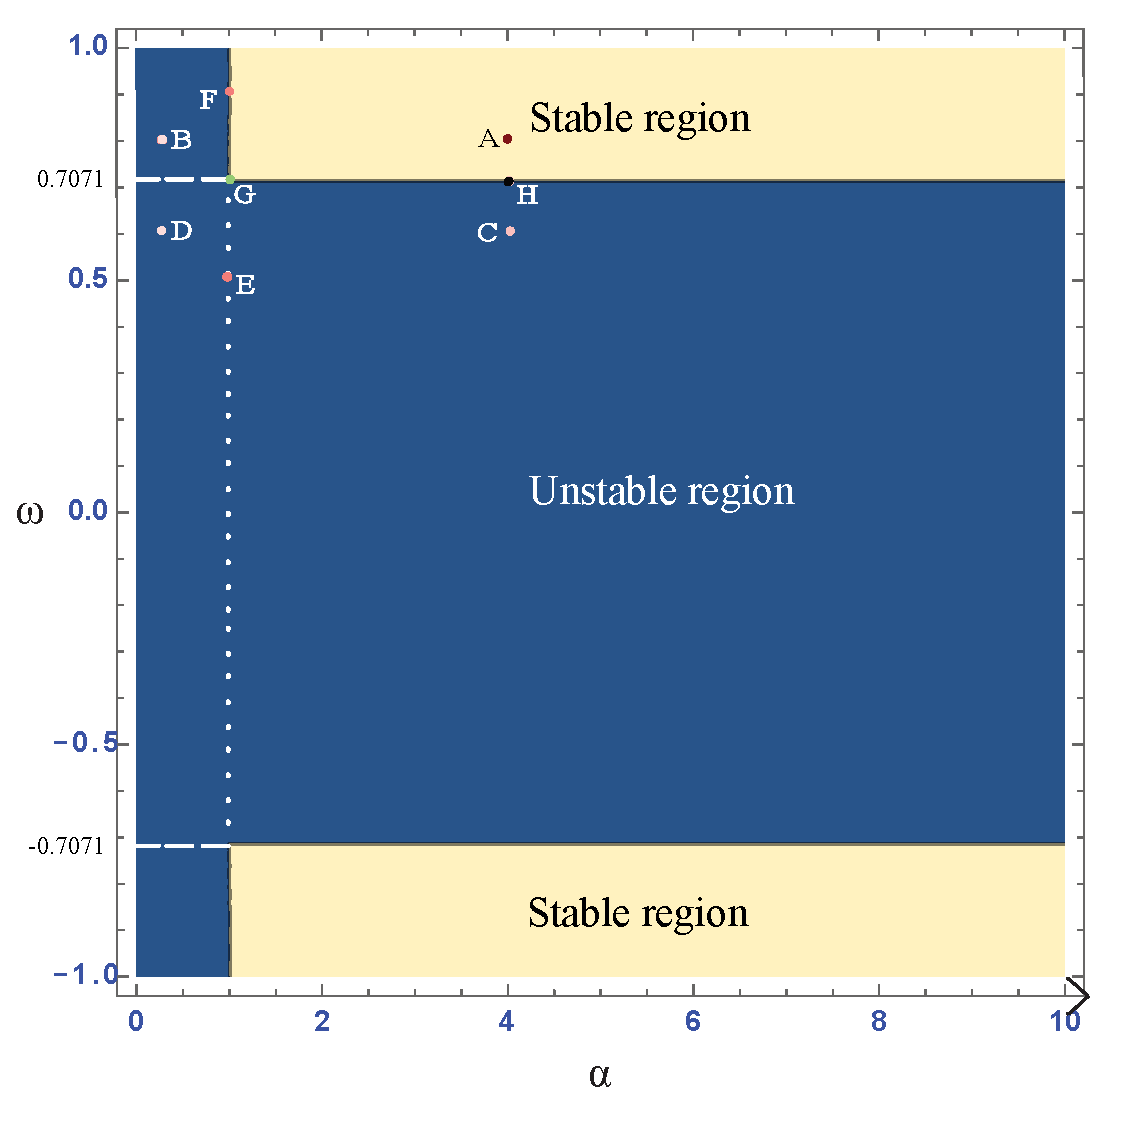
\includegraphics[width=1.0\textwidth]{Bifurcationavsw}
\caption[Bifurcation diagram a vs w]{The plot of the Stability region of Equilibrium points.}
\label{fig:Bifurcation a vs w}
\end{figure}

    %----------------------------------------------
\subsubsection{Discussion on the stability of the equilibrium points we obtained in the section \ref{Equilibrium-points}}\label{Discussion on the stability of the equilibrium points we obtained in the section}

In section \ref{Equilibrium-points} we obtained the equilibrium points in two cases.

\textbf{(i) $k=0$ or $|s|=\frac{1}{\sqrt{2}}$:} We obtain equilibrium points (\ref{line eq points}) only when s and w are of the same sign. (Note: A straight line parallel to the y-axis is the set of equilibrium points.)

\textit{Observations:} Eigenvalues of the coefficient matrix $A$ are of the form $a$, $b$, and $0$, where both a and b are complex numbers repeated with multiplicity two and $0$ has multiplicity 4. 
For $\alpha<1$, the point is on the dashed line where the equilibrium points are not unique, and the equilibrium is always unstable. $\alpha>1$ is on the solid line, which separates the stable and unstable region (bifurcation line); when $\alpha>1.6$, the eigenvalues are all real.  If $\alpha \in (0,1.6)$ a and b are complex conjugates.

\textbf{(ii) $det(\mathbb{G}_{0})\neq 0 $:}
The system is consistent and has unique solution, as in equation (\ref{unique eq point}).
The equilibrium point is stable if $\alpha>1$ and $\vert \omega\vert >\frac{1}{\sqrt{2}}$. Then the eigenvalue with the smallest argument will be in the stable region of the complex plane. The equilibrium point is unstable if $\alpha<1$ or $\vert\omega\vert <\frac{1}{\sqrt{2}}$ then at-least one eigenvalue will be in the unstable region of complex plane.

It is a well-established fact that a fractional-order system cannot have a periodic solution \cite{kaslik2012non}. It will have a solution tending to a closed orbit if the solution is stable, (i.e. limit cycle). The solutions for $\alpha=1$ and $\omega>1/\sqrt{2}$, are depicted in Fig. \ref{fig: Stable parametric Point F}.
%-----------------------------------------------------------------------------------------------------------------------------------------------------------------
\section{Some Particular Cases}\label{Some Particular cases}
In this section, we will discuss the stability of equilibrium points corresponding to the points in the bifurcation diagram (cf. Fig. \ref{fig:Bifurcation a vs w}).

\subsubsection{$1^{st}$ set of parameters: corresponding to point A in the bifurcation diagram.}
\label{$1{st}$ set}

For the parameter values $\alpha = 4$, $Re_{s}=0.05$, $\omega=0.8$, $k=0$ and $s=0.6$ eigenvalues are: $ \{\{-1.93195 \mp 0.0104183 i\},\{-0.517921 \mp 0.0205607 i\},\{-0.0499598\mp 0.0524144 i\},\{0.0503416\, \mp 0.0492603 i\}\}$.
The corresponding angles are : \\$\vert Arg(\lambda_{i})\vert - \frac{\pi}{4}= \{\{2.35458\},\{2.35017\},\{1.56834\},\{0.00195268\}\}$. Hence all the eigenvalues subtend angles greater than $\frac{\pi}{4}$.

From equation (\ref{unique eq point}) we get,
$$\mathbf{x}_{eq}=
\left(
\begin{array}{c}
 -857.076 \\
 19.9984 \\
\end{array}
\right).$$
For a particle released from
\begin{align*}
X_{0}=&
\left(
x(0) ,
y(0) ,
{ }_{0}^{C}D_{t}^{\frac{1}{2}}x(0) ,
{ }_{0}^{C}D_{t}^{\frac{1}{2}}y(0) ,
{ }_{0}^{C}D_{t}^{1} x(0) ,
{ }_{0}^{C}D_{t}^{1}y(0) ,
{ }_{0}^{C}D_{t}^{\frac{3}{2}}x(0) ,
{ }_{0}^{C}D_{t}^{\frac{3}{2}}y(0)
\right)^T \\ =& \left(
 -856.393,
 20.5373,
 0.884826,
 0.318784,
 0.888572,
 0.713742,
 0.907138,
 0.999199 
\right),
\end{align*}
the solution has a self-intersecting trajectory which converges to the equilibrium point. The solution curves are plotted in Fig. \ref{fig:Stable parametric corresponding to point A on bifurcation diagram} and Fig. \ref{fig:Stable case corresponding to point A on bifurcation diagram}.

\begin{figure}[h]%
\centering
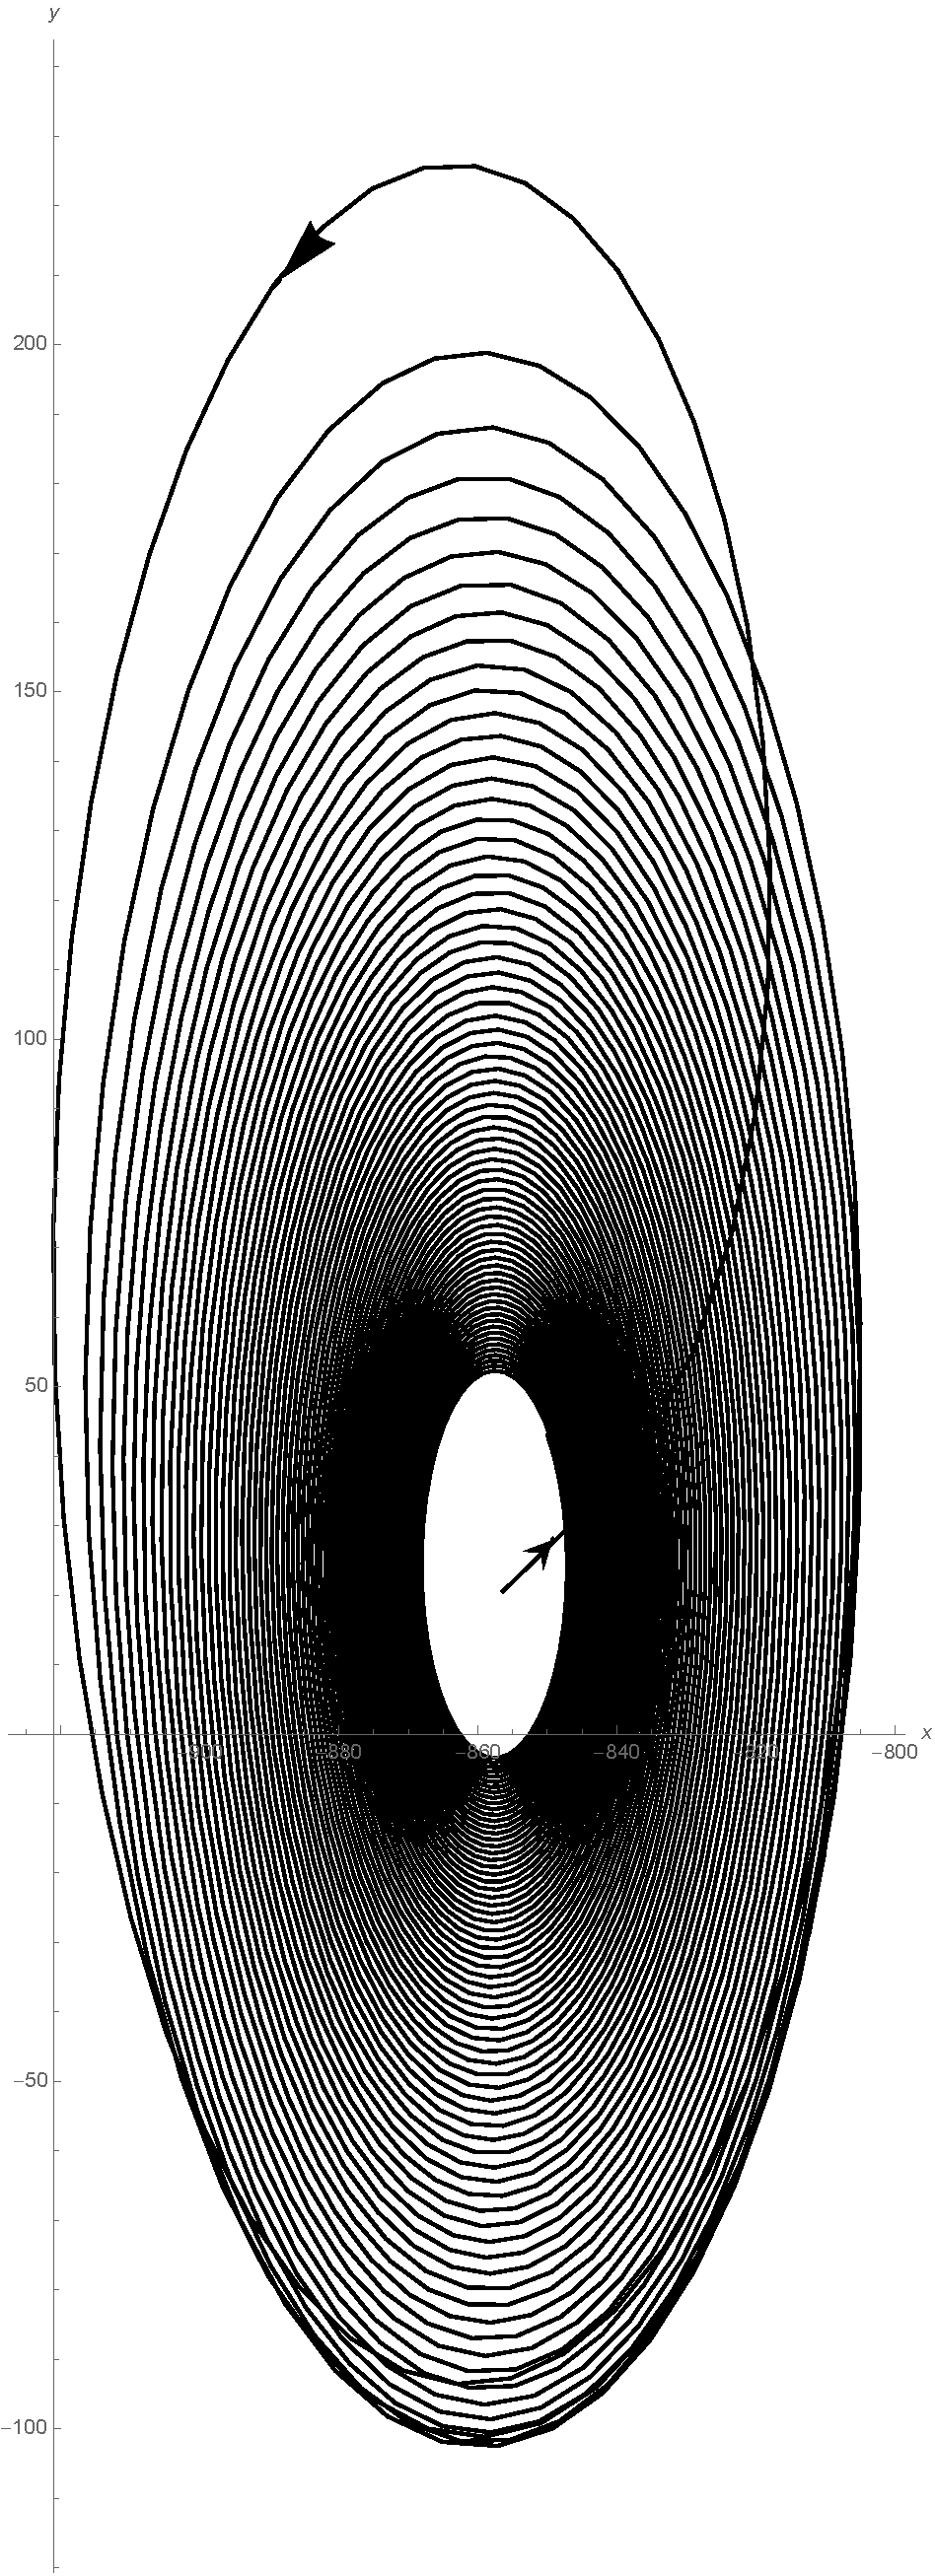
\includegraphics[width=0.3\textwidth]{Fig2left(stable)Parametric}
    \caption{Parametric plot of solution for  $k=0$ and $ s=0.6$. This stable case corresponds to point A on bifurcation diagram, $\alpha = 4$ and  $\omega = 0.8$.}
    \label{fig:Stable parametric corresponding to point A on bifurcation diagram}
\end{figure}
\begin{figure}[h]%
\centering
 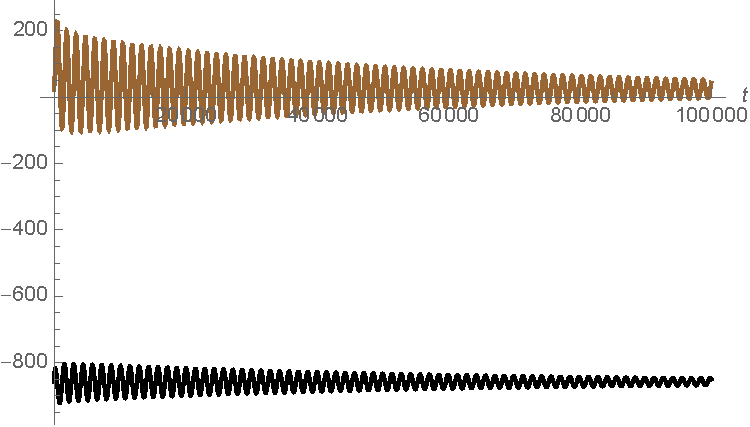
\includegraphics[width=0.4\textwidth]{Fig2left(stablePlot}
    \caption{Plot of x and y vs time for $k = 0$ and $s = 0.6$. This stable case corresponds to point A on bifurcation diagram, $\alpha = 4$ and  $\omega = 0.8$.}
    \label{fig:Stable case corresponding to point A on bifurcation diagram}
\end{figure}

\subsubsection{$2^{nd}$ set of parameters: corresponding to point A in the bifurcation diagram.} \label{$2{nd}$ set}

For the parameter values $\alpha = 4$, $Re_{s}=0.05$, $\omega=0.8,s=0,k=0.6$
the eigenvalues are independent of $s$, and $k$  will be the same as in the $1^{st}$ set of parameters and thus stable.

In this case using equation (\ref{unique eq point}) we get,
$$\mathbf{x}_{eq}=
\left(
\begin{array}{c}
 -3428.3 \\
 -2551.23 \\
\end{array}
\right).$$
If we set
\begin{align*}
X_{0}=&
\left(
x(0),
y(0),
{ }_{0}^{C}D_{t}^{\frac{1}{2}}x(0),
{ }_{0}^{C}D_{t}^{\frac{1}{2}}y(0),
{ }_{0}^{C}D_{t}^{1} x(0),
{ }_{0}^{C}D_{t}^{1}y(0),
{ }_{0}^{C}D_{t}^{\frac{3}{2}}x(0),
{ }_{0}^{C}D_{t}^{\frac{3}{2}}y(0)
\right)^T, \\ =& \left(
 -3428.11,
 -2550.41,
 0.678964,
 0.346004,
 0.0456744,
 0.262553,
 0.51563,
 0.782148 
\right) 
\end{align*}
then, the solution obtained has a self-intersecting trajectory that converges to the equilibrium point as in the previous case (Fig. \ref{fig:Stable parametric s,k,Stable case corresponding to point A on bifurcation diagram} and Fig. \ref{fig:Stale s,k,Stable case corresponding to point A on bifurcation diagram}). 

Note that the parameters $s$ and $k$ do not affect the stability. However, they play a role in the equilibrium point's position and decide the orientation of the elliptical spiral orbit in phase space (cf. Fig.\ref{fig:Stable parametric corresponding to point A on bifurcation diagram}  and Fig. \ref{fig:Stable parametric s,k,Stable case corresponding to point A on bifurcation diagram}).

\begin{figure}[h]%
\centering
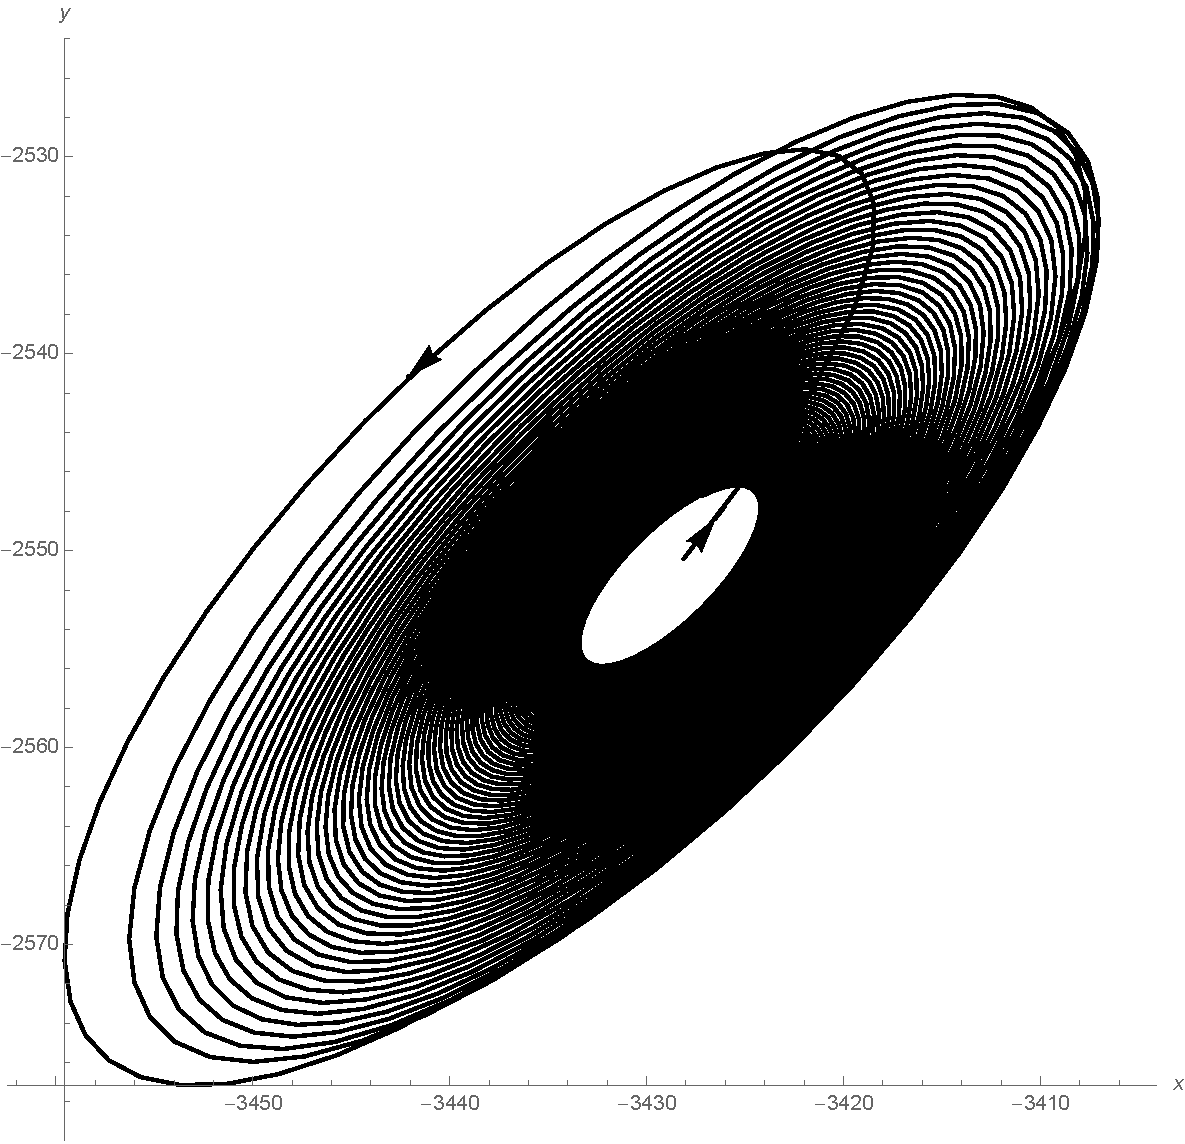
\includegraphics[width=0.4\textwidth]{Fig2right(stable)Parametric}
    \caption{Parametric plot of solution for  $s=0$ and $ k=0.6$. This stable case corresponds to point A on bifurcation diagram, $\alpha = 4$ and  $\omega = 0.8$.}
    \label{fig:Stable parametric s,k,Stable case corresponding to point A on bifurcation diagram}
\end{figure}
\begin{figure}[h]%
\centering
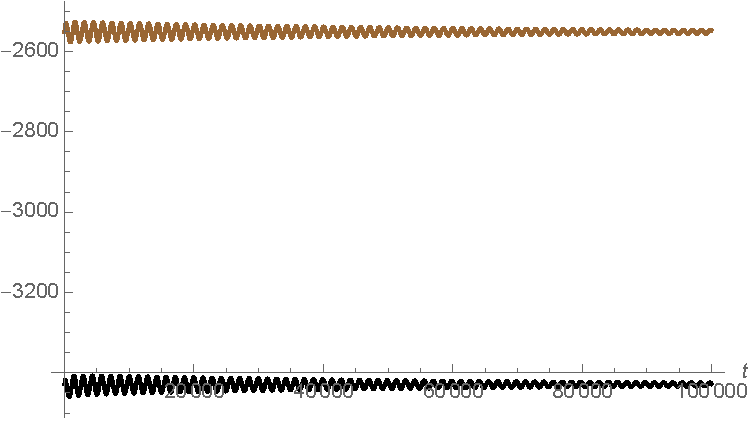
\includegraphics[width=0.4\textwidth]{Fig2right(stable)Plot}
    \caption{Plot of x and y vs time for $s = 0$ and $k = 0.6$. This stable case corresponds to point A on bifurcation diagram, $\alpha = 4$ and  $\omega = 0.8$.}
    \label{fig:Stale s,k,Stable case corresponding to point A on bifurcation diagram}
\end{figure}


\subsubsection{$3^{rd}$ set of parameters: corresponding to point B in the bifurcation diagram.} \label{$3^{rd}$ set}
Consider,  $\alpha = \frac{1}{4}$,  $Re_{s}=0.05$,  $\omega=0.8$, $k=0$ and $s=0.6$ which corresponds to point B in Fig \ref{fig:Bifurcation a vs w}, which is in the unstable region.

The eigenvalues of matrix A with this set of parameters are: $\{-0.515042 \pm 0.866277 i, -0.484494 \pm 0.866314 i,-0.116242 \pm 0.11396 i, 0.115777 \pm 0.113997 i\}$

$\therefore \vert Arg(\lambda_{i})\vert -\frac{\pi}{4}=\{1.3218,1.29532,1.58071,-0.00774575,\}$. So the last two eigenvalues subtend angle less than $\frac{\pi}{4}$ that makes it unstable.

In this case,
$$\mathbf{x}_{eq}=
\left(
\begin{array}{c}
 142.846 \\
-3.33307 \\
\end{array}
\right).$$
If we set 
\begin{align*}
X_{0}=&
\left(
x(0) ,
y(0) ,
{ }_{0}^{C}D_{t}^{\frac{1}{2}}x(0) ,
{ }_{0}^{C}D_{t}^{\frac{1}{2}}y(0) ,
{ }_{0}^{C}D_{t}^{1} x(0) ,
{ }_{0}^{C}D_{t}^{1}y(0) ,
{ }_{0}^{C}D_{t}^{\frac{3}{2}}x(0) ,
{ }_{0}^{C}D_{t}^{\frac{3}{2}}y(0)
\right)^T, \\ =& \left(
 143.756,
 -2.581,
 0.866811,
 0.513388,
 0.761374,
 0.983692,
 0.84388,
 0.73129 
\right)
\end{align*} 
then, the particle diverges away from the equilibrium point by travelling in an elliptical spiral path (cf. Fig.\ref{fig: Unstable parametric case corresponding to point B on bifurcation diagram} and Fig.\ref{fig: Unstable case corresponding to point B on bifurcation diagram}). This is consistent with the stability analysis presented in section \ref{Stability and Bifurcation Analysis}.

\begin{figure}[h]%
\centering
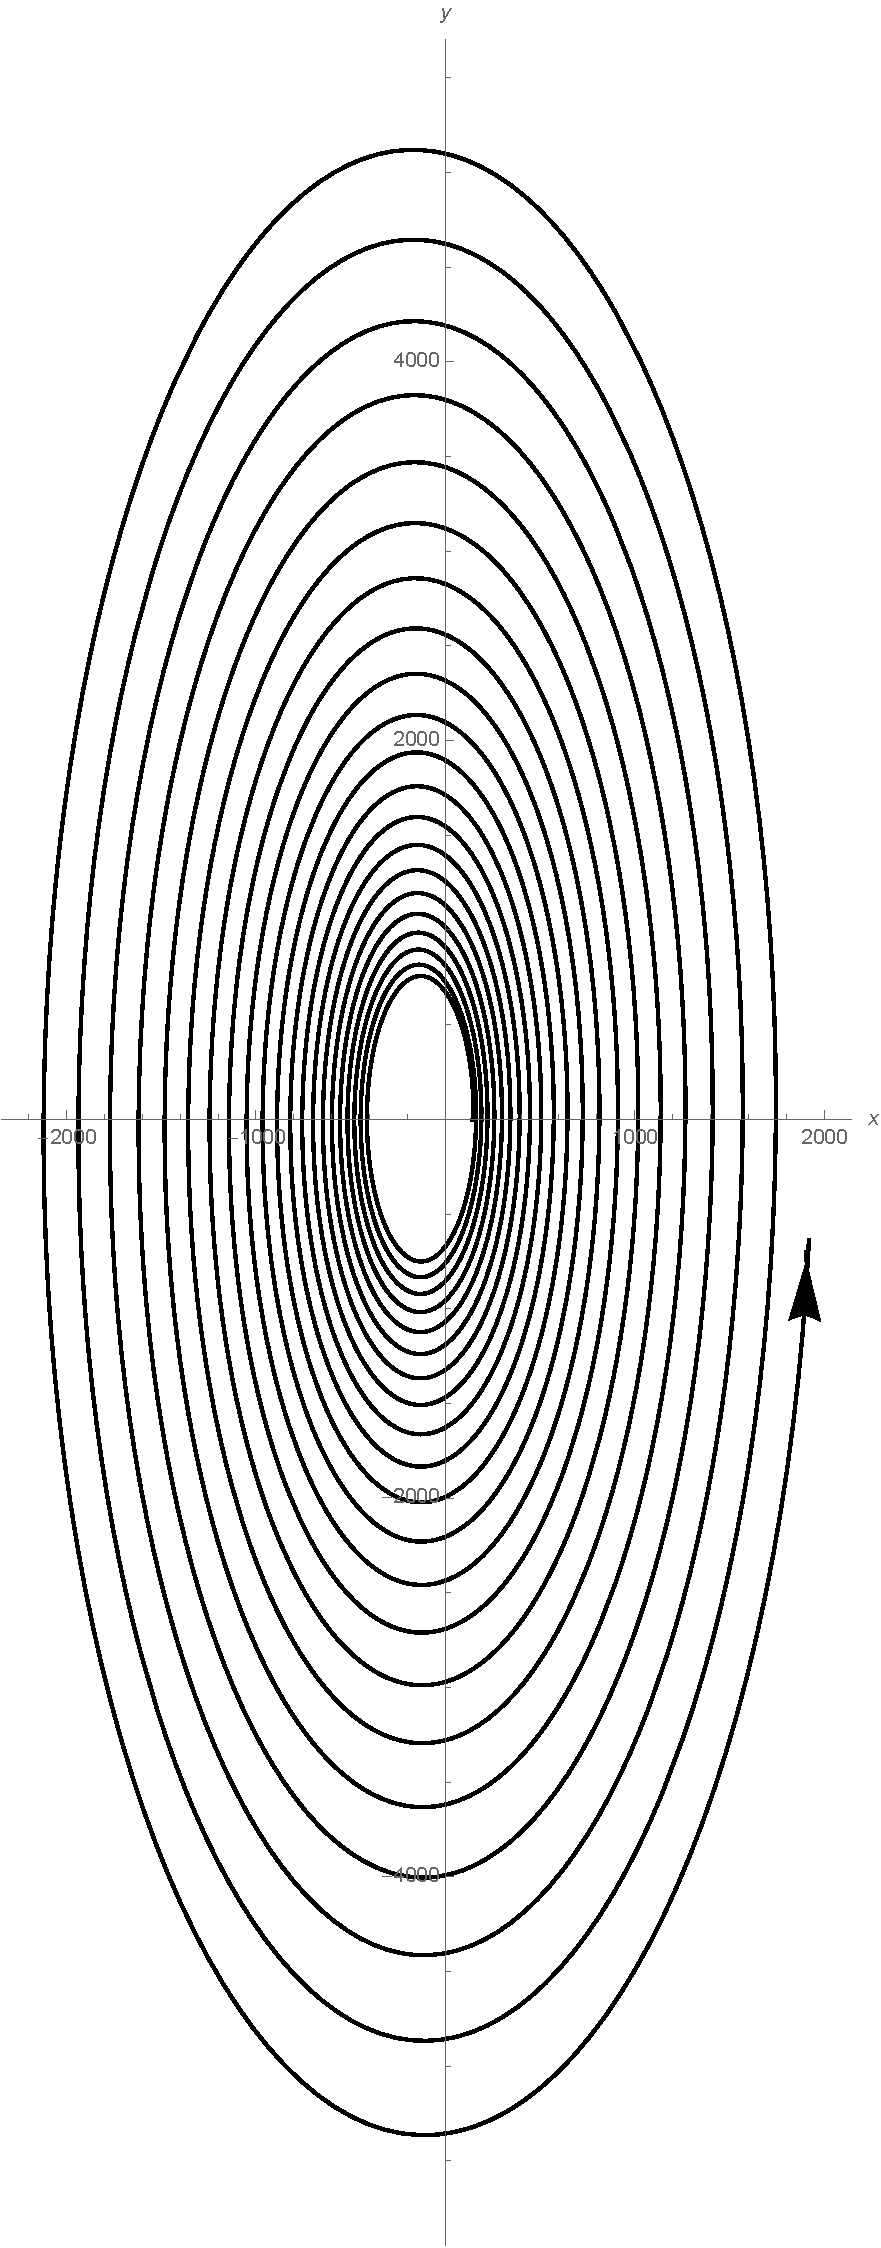
\includegraphics[width=0.3\textwidth]{Fig3left(unstable)Parametric}
    \caption{Parametric plot of (unstable) solution corresponding to point B on the bifurcation diagram  $\alpha = \frac{1}{4}$, $\omega = 0.8$, $k=0$ and $s=0.6$.}
    \label{fig: Unstable parametric case corresponding to point B on bifurcation diagram}
\end{figure}
\begin{figure}[h]%
\centering
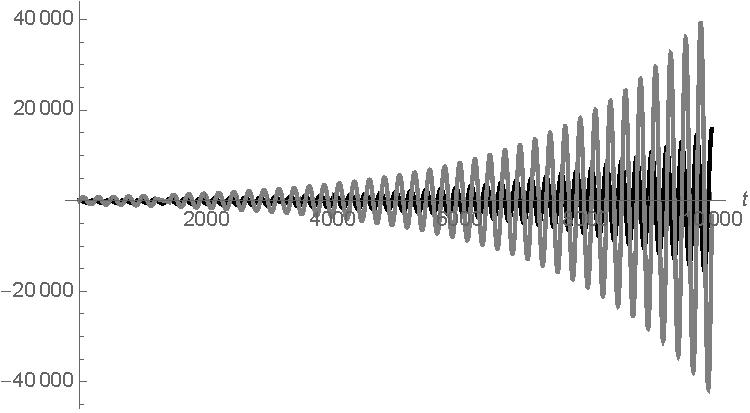
\includegraphics[width=0.4\textwidth]{Fig3left(unstable)plot}
    \caption{Plot of $x$ and $y$ vs time corresponding to point B on the bifurcation diagram $\alpha = \frac{1}{4}$, $\omega = 0.8$, $k=0$ and $s=0.6$.}
        \label{fig: Unstable case corresponding to point B on bifurcation diagram}
\end{figure}



\subsubsection{$4^{th}$ set of parameters: corresponding to point B in the bifurcation diagram.} \label{$4^{th}$ set}

Let us consider $\alpha = \frac{1}{4}$, $Re_{s}=0.05$,  $\omega=0.8$, $s=0$ and $k=0.6$. For this parameter set,  as the eigenvalues of A are independent of $s$ and $k$ and hence will be the same as the $3^{rd}$ set of parameters and hence unstable.

The equilibrium point in this case is
$\mathbf{x}_{eq}=
\left(
\begin{array}{c}
 -571.384 \\
-425.205 \\
\end{array}
\right)$.

For the initial condition, \begin{align*}
X_{0}=&
\left(
x(0) ,
y(0) ,
{ }_{0}^{C}D_{t}^{\frac{1}{2}}x(0) ,
{ }_{0}^{C}D_{t}^{\frac{1}{2}}y(0) ,
{ }_{0}^{C}D_{t}^{1} x(0) ,
{ }_{0}^{C}D_{t}^{1}y(0) ,
{ }_{0}^{C}D_{t}^{\frac{3}{2}}x(0) ,
{ }_{0}^{C}D_{t}^{\frac{3}{2}}y(0)
\right)^T \\ =& \left(
 -571.213,
 -424.231,
 0.779817,
 0.485663,
 0.717887,
 0.82599,
 0.259935,
 0.811328 
\right),
\end{align*}
the particle diverges away from the equilibrium point by travelling in an elliptical spiral path (See figures Fig. \ref{fig:Unstable parametric s,k corresponding to point B on bifurcation diagram} and Fig. \ref{fig:Unstale s,k. corresponding to point B on bifurcation diagram}). Note that here $s$ and $k$ have no part in stability. However, they play a role in the equilibrium position and the elliptical spiral's orientation. Observe the difference in orientation concerning the $3^{rd}$ set of parameters. 
\begin{figure}[h]%
\centering
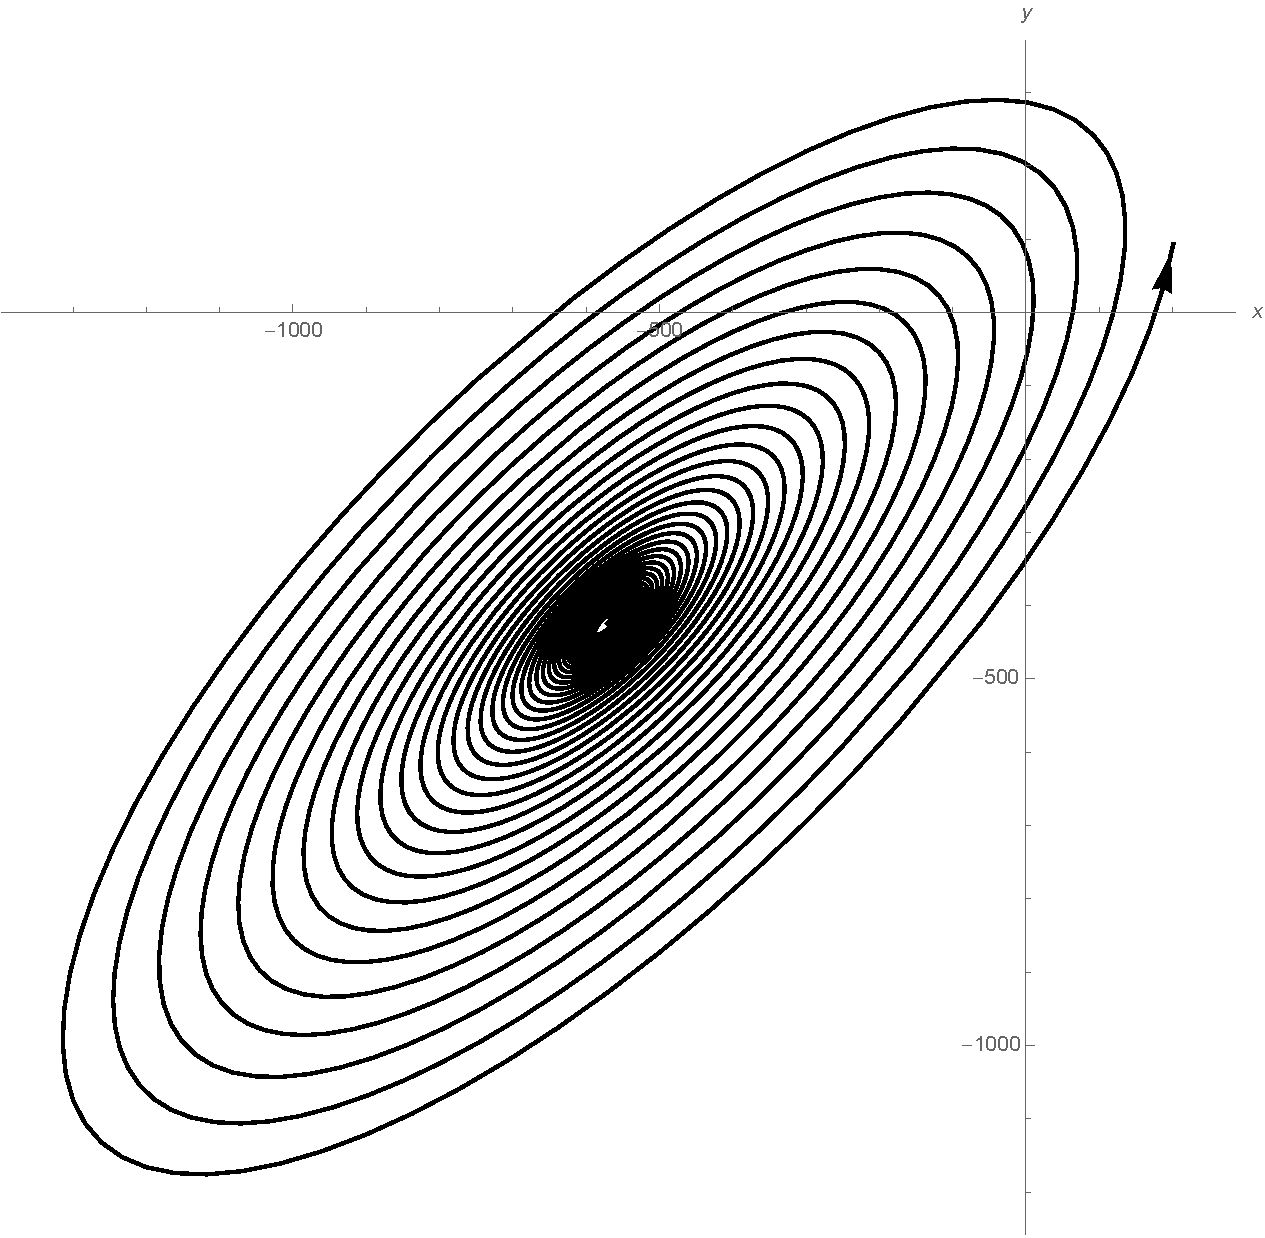
\includegraphics[width=0.4\textwidth]{Fig3right(unstable)Parametric}
    \caption{Parametric plot of (unstable) solution corresponding to point C on the bifurcation diagram  $\alpha = \frac{1}{4}$, $\omega = 0.8$, $s=0$ and $ k=0.6$.}
    \label{fig:Unstable parametric s,k corresponding to point B on bifurcation diagram}
\end{figure}
\begin{figure}[h]%
\centering
      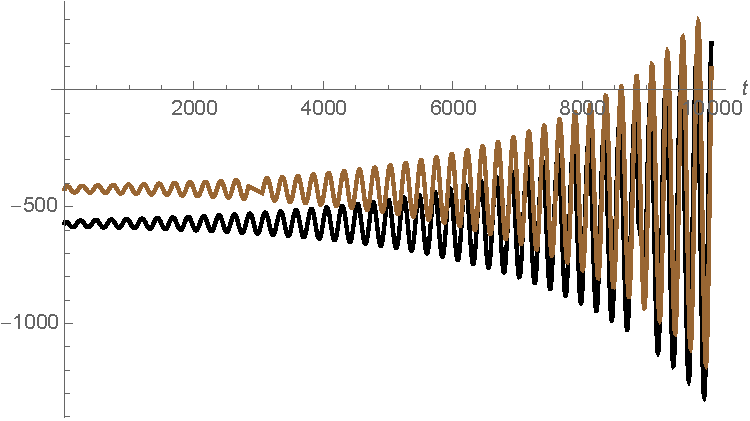
\includegraphics[width=0.4\textwidth]{Fig3right(unstable)plot}
    \caption{Parametric plot of (unstable) solution corresponding to point B on the bifurcation diagram  $\alpha = \frac{1}{4}$, $\omega = 0.8$, $s=0$ and $k=0.6$.}
    \label{fig:Unstale s,k. corresponding to point B on bifurcation diagram}
\end{figure}

\subsubsection{$5^{th}$ set of parameters: corresponding to point C in the bifurcation diagram.}\label{$5^{th}$ set}

The values $\alpha = 4$, $Re_{s}=0.05$, $\omega=0.6$,  $s=0.8$ and $k=0$ correspond to the point C in Fig. \ref{fig:Bifurcation a vs w}.

The eigenvalues corresponding to this point are, $\{-1.93497,-1.92873,-0.520711,-0.514476, -0.0665776,-0.0000236085 \mp0.0662607 i,0.0665295\}$
with corresponding angles : $\vert Arg(\lambda_{i})\vert-\frac{\pi}{4} =\{\frac{3 \pi }{4},\frac{3 \pi }{4},\frac{3 \pi }{4},\frac{3 \pi }{4},\frac{3 \pi }{4},\mp 0.785754,-\frac{\pi }{4}\}$. The last eigenvalue is real and positive, due to which the system is unstable.

If the initial conditions are \begin{align*}
X_{0}=&
\left(
x(0) ,
y(0) ,
{ }_{0}^{C}D_{t}^{\frac{1}{2}}x(0) ,
{ }_{0}^{C}D_{t}^{\frac{1}{2}}y(0) ,
{ }_{0}^{C}D_{t}^{1} x(0) ,
{ }_{0}^{C}D_{t}^{1}y(0) ,
{ }_{0}^{C}D_{t}^{\frac{3}{2}}x(0) ,
{ }_{0}^{C}D_{t}^{\frac{3}{2}}y(0)
\right)^T \\ =& \left(
 -856.895,
 20.857,
 0.383745,
 0.813572,
 0.611775,
 0.768673,
 0.968454,
 0.24313 
\right),
\end{align*}
 then, we observe in Fig. \ref{fig:Unstable parametric case corresponding to point C on bifurcation diagram} and Fig. \ref{fig:Unstable Plot case corresponding to point C on bifurcation diagram}  that the particle diverges away from the equilibrium point, as predicted (cf. section \ref{Stability and Bifurcation Analysis}).

\begin{figure}
  \centering
    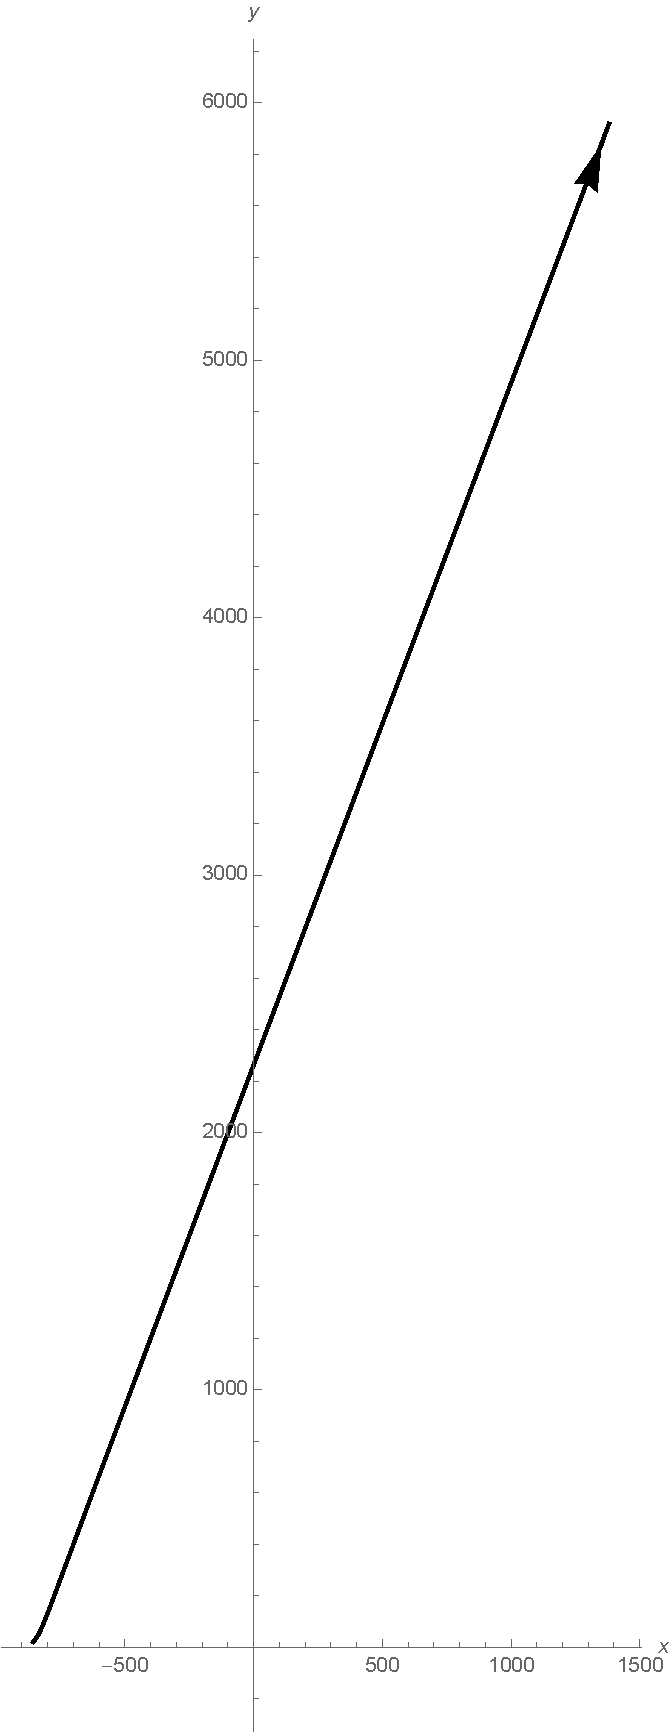
\includegraphics[width=0.25\textwidth]{Fig4Right(unstable)Parametric}
    \caption{Parametric plot of (unstable) solution corresponding to point C on the bifurcation diagram $\alpha = 4$, $\omega = 0.6$, $s=0.8$ and $k=0$.}
    \label{fig:Unstable parametric case corresponding to point C on bifurcation diagram}   
\end{figure}
\begin{figure}[h]%
\centering
    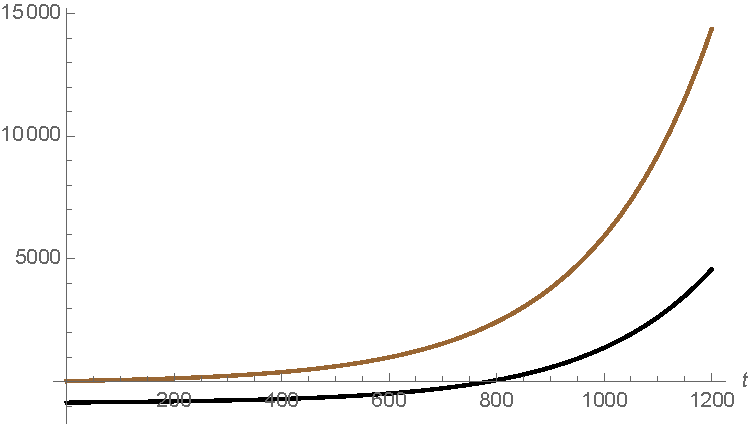
\includegraphics[width=0.4\textwidth]{Fig4right(unstable)plot}
    \caption{Plot of $x$ and $y$ vs $t$ corresponding to point C on the bifurcation diagram $\alpha = 4$, $\omega = 0.6$, $s=0.8$ and $k=0$.}
    \label{fig:Unstable Plot case corresponding to point C on bifurcation diagram}
\end{figure}

\subsubsection{$6^{th}$ set of parameters: corresponding to point D in the bifurcation diagram.}\label{$6{th}$ set}
The parameter values $\alpha = 1/4$, $Re_{s}=0.05$, $\omega=0.6$, $s=0.8$ and $k=0$ represent point D in Fig \ref{fig:Bifurcation a vs w}.

Corresponding to point D the eigenvalues are: $\{ -0.500253 \pm 0.85048i,  -0.500216 \pm 0.881033i,  -0.16104, 0.000252788 \pm 0.164122i, 0.161472 \}$
the corresponding angles are,
$\vert Arg(\lambda_{i})\vert -\frac{\pi}{4}=\{1.3171, 1.30177,\frac{3\pi}{4},0.783858,-\frac{\pi}{4}\}$. The last eigenvalue is real and positive, due to which the system is unstable.
Here, we get the equilibrium point as
$$\mathbf{x}_{eq}=
\left(
\begin{array}{c}
 -571.384 \\
-425.205 \\
\end{array}
\right)$$

If we have the initial condition as \begin{align*}
X_{0}=&
\left(
x(0) ,
y(0) ,
{ }_{0}^{C}D_{t}^{\frac{1}{2}}x(0) ,
{ }_{0}^{C}D_{t}^{\frac{1}{2}}y(0) ,
{ }_{0}^{C}D_{t}^{1} x(0) ,
{ }_{0}^{C}D_{t}^{1}y(0) ,
{ }_{0}^{C}D_{t}^{\frac{3}{2}}x(0) ,
{ }_{0}^{C}D_{t}^{\frac{3}{2}}y(0)
\right)^T \\ =& \left(
 -142.63,
 3.81508,
 0.0751995,
 0.8842,
 0.758708,
 0.803567,
 0.911143 ,
 0.47276,
\right)^T
\end{align*}
We obtain the solution where the particle diverges from the equilibrium point as depicted in Fig. \ref{fig:Unstable parametric Point D} and Fig. \ref{fig:Unstable  Point D}.

\begin{figure}
  \centering
    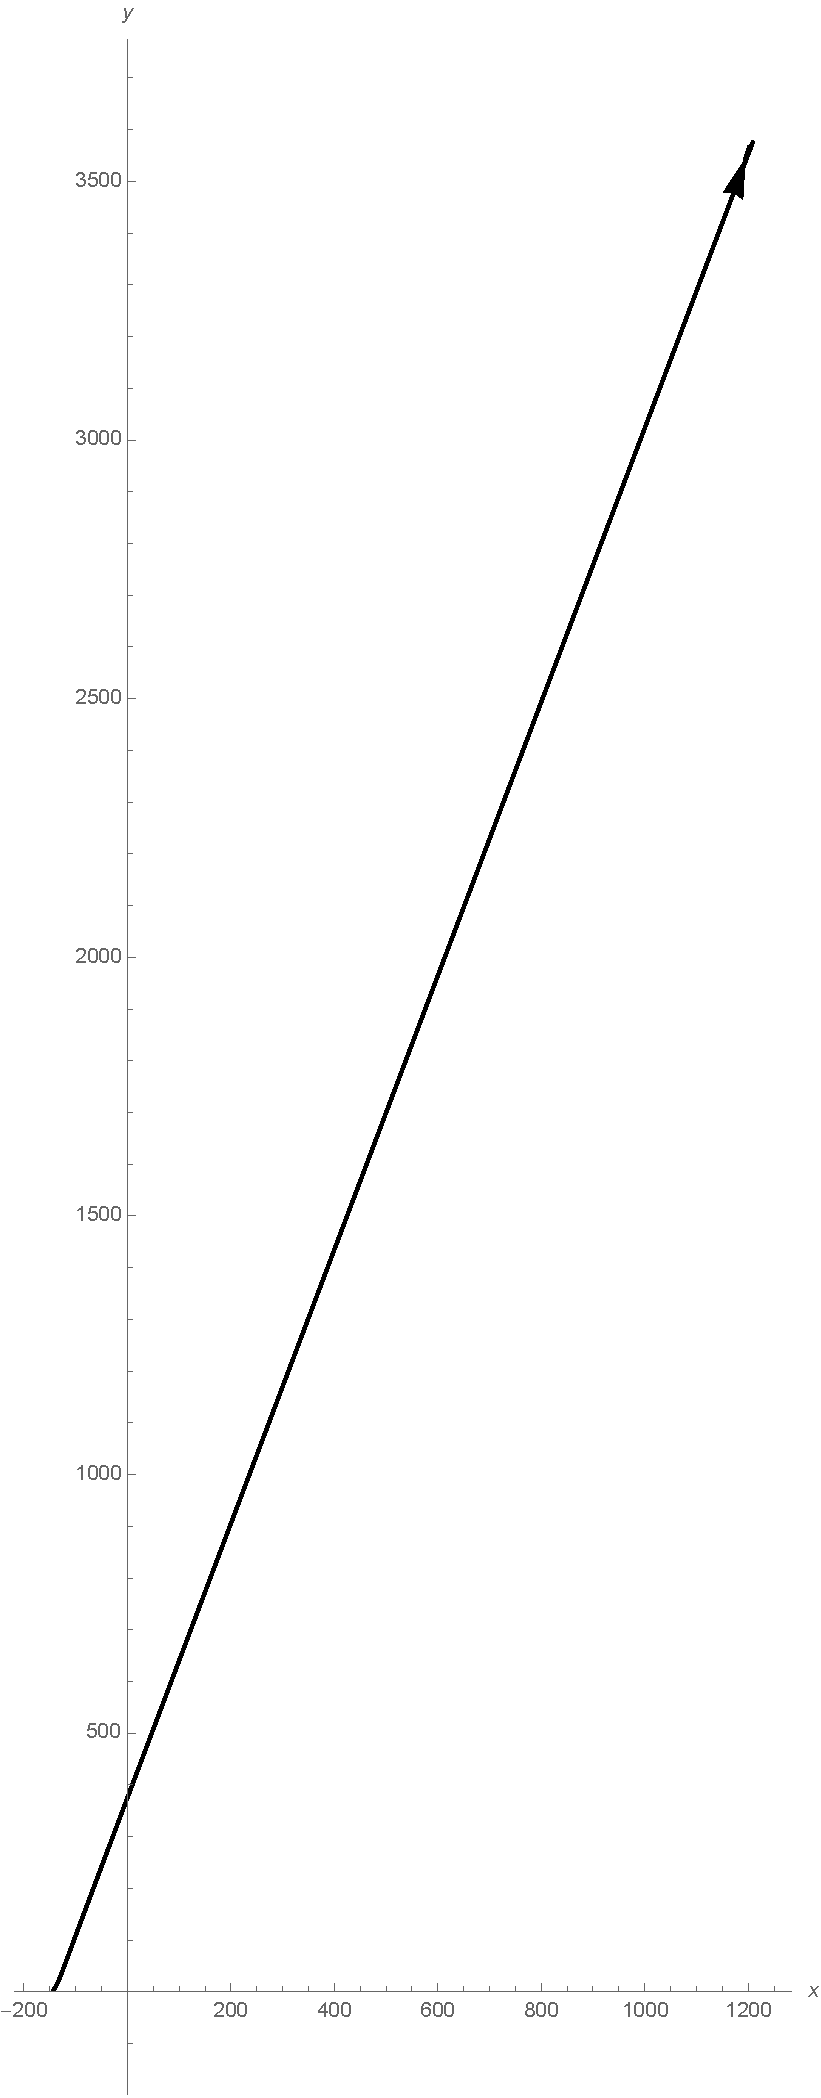
\includegraphics[width=0.25\textwidth]{Fig4Left(unstable)Parametric}
    \caption{Parametric plot of (unstable) solution corresponding to point D on the bifurcation diagram, $\alpha = \frac{1}{4}$,  $\omega = 0.6$.  $s=0.8$ and $k=0$. }
    \label{fig:Unstable parametric Point D}   
\end{figure}

\begin{figure}[h]%
\centering
  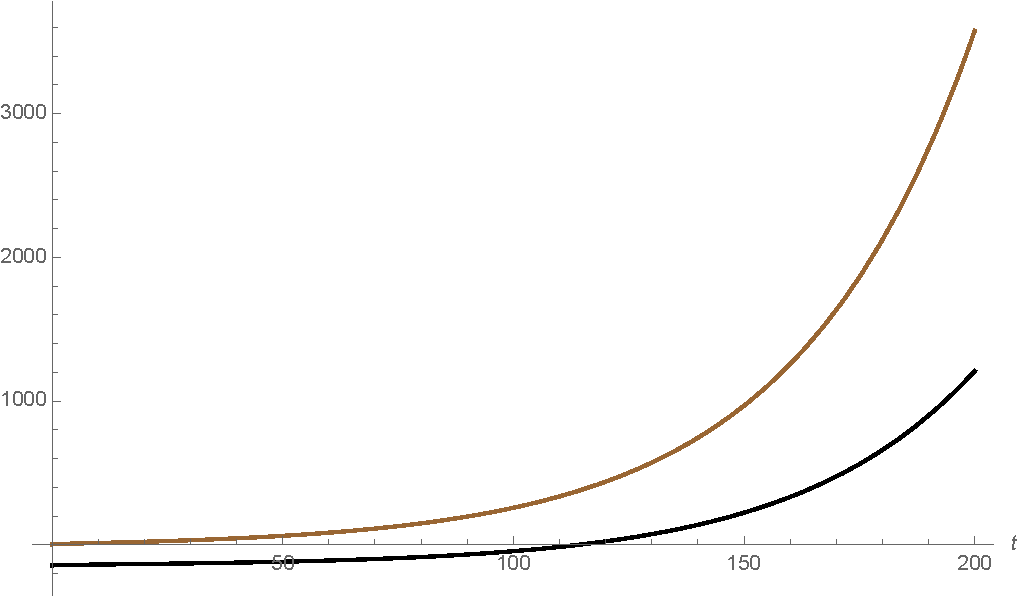
\includegraphics[width=0.4\textwidth]{Fig4Left(unstable)Plot}
    \caption{Plot of $x$ and $y$ vs $t$ corresponding to point D on the bifurcation diagram, $\alpha = \frac{1}{4}$,  $\omega = 0.6$.  $s=0.8$ and $k=0$.}
    \label{fig:Unstable  Point D}
\end{figure}

\subsubsection{$7^{th}$ set of parameters: corresponding to point E in the bifurcation diagram.}\label{$7{th}$ set}
Assume that, $\alpha = 1$, $Re_{s}=0.05$, $\omega=0.5$, $s=0.7071$ and $k=0.5$. This corresponds to the point E in Fig \ref{fig:Bifurcation a vs w}.

Corresponding to E, the eigenvalues are, $\{-0.866025 \pm 0.488073 i,-0.866025 \pm 0.511649 i,-0.108559,0.\pm 0.108559 i,0.108559\}$
with corresponding angles:  $\vert Arg(\lambda_{i})\vert - \frac{\pi}{4}= \{1.07267,1.07247,\frac{3 \pi}{4},0.796945, -\frac{\pi}{4}\}$. As the last eigenvalue is real and positive, the system is unstable.  

The equilibrium point is, $$\mathbf{x}_{eq}=\left(
\begin{array}{c}
 -248.563 \\
610.085\\
\end{array}
\right).$$ 

 With the initial condition, \begin{align*}
X_{0}=&
\left(
x(0) ,
y(0) ,
{ }_{0}^{C}D_{t}^{\frac{1}{2}}x(0) ,
{ }_{0}^{C}D_{t}^{\frac{1}{2}}y(0) ,
{ }_{0}^{C}D_{t}^{1} x(0) ,
{ }_{0}^{C}D_{t}^{1}y(0) ,
{ }_{0}^{C}D_{t}^{\frac{3}{2}}x(0) ,
{ }_{0}^{C}D_{t}^{\frac{3}{2}}y(0)
\right)^T \\ =& \left(
 -247.597,
 610.322,
 0.0108669,
 0.0186482,
 0.0144648,
 0.897224,
 0.762554,
 0.460495 
\right)^T,
\end{align*} we can observe in Fig. \ref{fig:Unstable parametric Point E} and Fig. \ref{fig:Unstable  Point E} that the solution trajectory of the particle diverges away from the equilibrium point as mentioned previously.  

  \begin{figure}
  \centering
    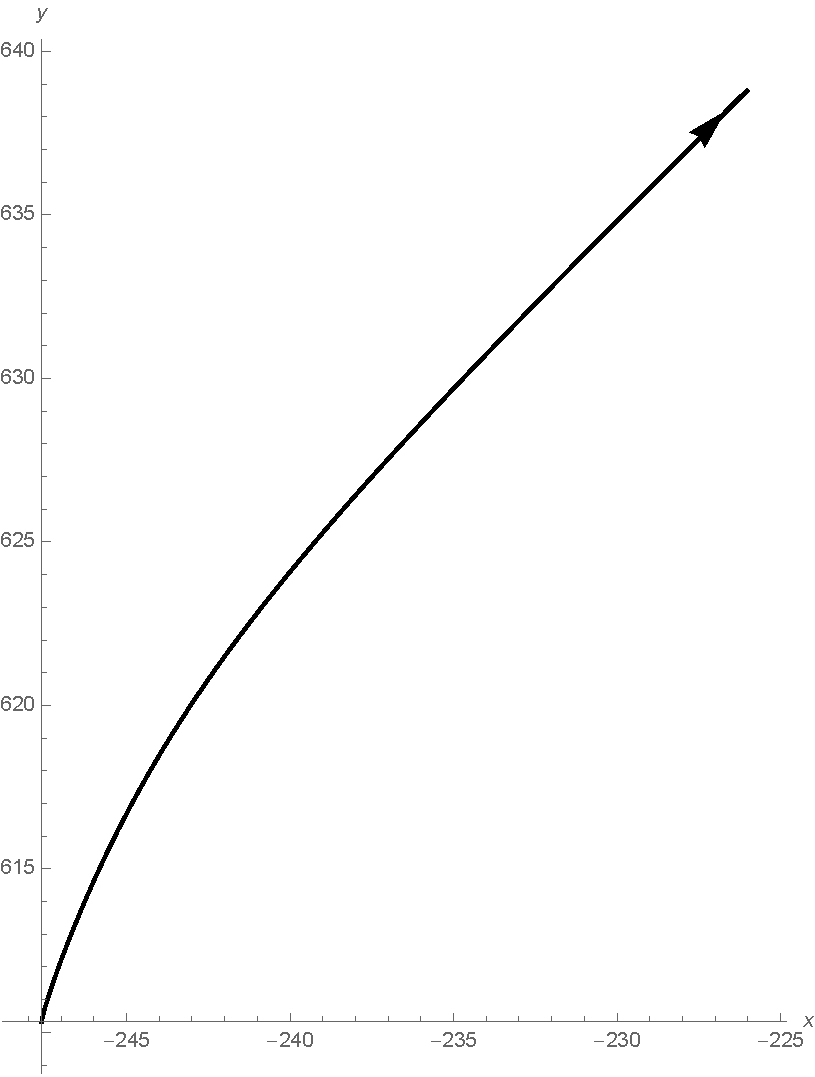
\includegraphics[width=0.3\textwidth]{Unstable_ais1Para}
    \caption{Parametric plot (unstable) solution  case corresponding to point E on bifurcation diagram, $\alpha = 1$, $\omega=0.5$, $s=0.7071$ and $k=0.5$.}
    \label{fig:Unstable parametric Point E}   
\end{figure} 

\begin{figure}[h]%
\centering
    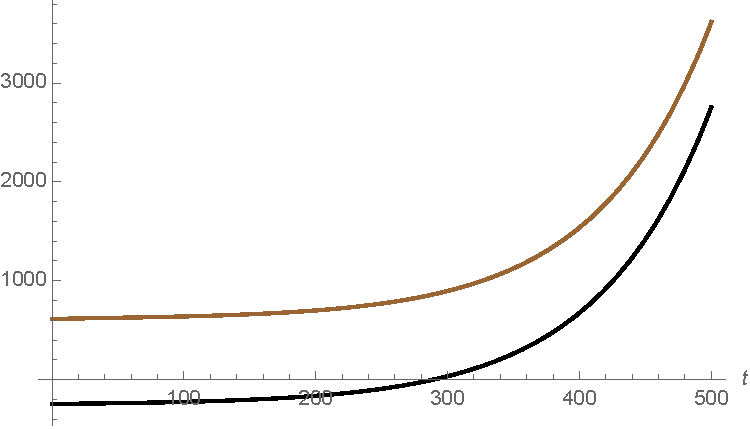
\includegraphics[width=0.4\textwidth]{Unstable_ais1Plot}
    \caption{Plot of $x$ and $y$ vs $t$ corresponding to point E on bifurcation diagram, $\alpha = 1$, $\omega=0.5$, $s=0.7071$ and $k=0.5$.}
    \label{fig:Unstable  Point E}
\end{figure}

\subsubsection{$8^{th}$ set of parameters: corresponding to point F in the bifurcation diagram.}\label{$8{th}$ set}
Corresponding to the point F (cf. Fig. \ref{fig:Bifurcation a vs w}) we consider,	$\alpha = 1$, $Re_{s}=0.05$, $\omega=0.9$, $s=0.424264$ and $k=0.1$.

Then we get the eigenvalues of matrix A as : $\{-0.879144 \pm 0.500172 i,-0.852907 \pm0.500172 i,-0.0810042 \pm 0.0810042 i,0.0810042 \pm 0.0810042 i\}$
with corresponding angles:  $\vert Arg(\lambda_{i})\vert - \frac{\pi}{4}= \{1.83893,1.82581,1.5708,0.\}$. The last two eigenvalues are on the boundary of the bifurcation curve in the complex plane.  In view of the discussion in section \ref{Stability and Bifurcation Analysis}, we get a stable trajectory converging to a closed orbit around the equilibrium point.

In this case, the equilibrium point is $$\mathbf{x}_{eq}=
\left(
\begin{array}{c}
 460.31 \\
86.7593\\
\end{array}
\right).$$

With the initial condition : \begin{align*}
X_{0}=&
\left(
x(0) ,
y(0) ,
{ }_{0}^{C}D_{t}^{\frac{1}{2}}x(0) ,
{ }_{0}^{C}D_{t}^{\frac{1}{2}}y(0) ,
{ }_{0}^{C}D_{t}^{1} x(0) ,
{ }_{0}^{C}D_{t}^{1}y(0) ,
{ }_{0}^{C}D_{t}^{\frac{3}{2}}x(0) ,
{ }_{0}^{C}D_{t}^{\frac{3}{2}}y(0)
\right)^T \\ =& \left(
 -459.949,
 -86.7209,
 0.535998,
 0.446247,
 0.80232,
 0.274064,
 0.126069,
 0.0023739 
 \right)^T,
\end{align*}
we obtain the solutions as depicted in Fig. \ref{fig: Stable parametric Point F} and Fig. \ref{fig:Stable  Point F}. Here the particle does not trace a closed orbit but will follow a trajectory which converges to a closed elliptical orbit. \\
$ x(t)=-460.31+0.506645 \left(2 y_{80} \cos (0.00656167 t)-2 y_{70} \sin (0.00656167 t)\right)$\\       \quad \quad $+0.064344 \left(2 y_{80} \sin (0.00656167 t)+2 y_{70} \cos (0.00656167 t)\right) $\\
$  y(t)=0.852084 \left(2 y_{80} \sin (0.00656167 t)+2 y_{70} \cos (0.00656167 t)\right)-86.7593$ \\ where $y_{70}={ }_{0}^{C}D_{t}^{\frac{3}{2}}x(0)$ and $y_{80}={ }_{0}^{C}D_{t}^{\frac{3}{2}}y(0)$.
  \begin{figure}
  \centering
    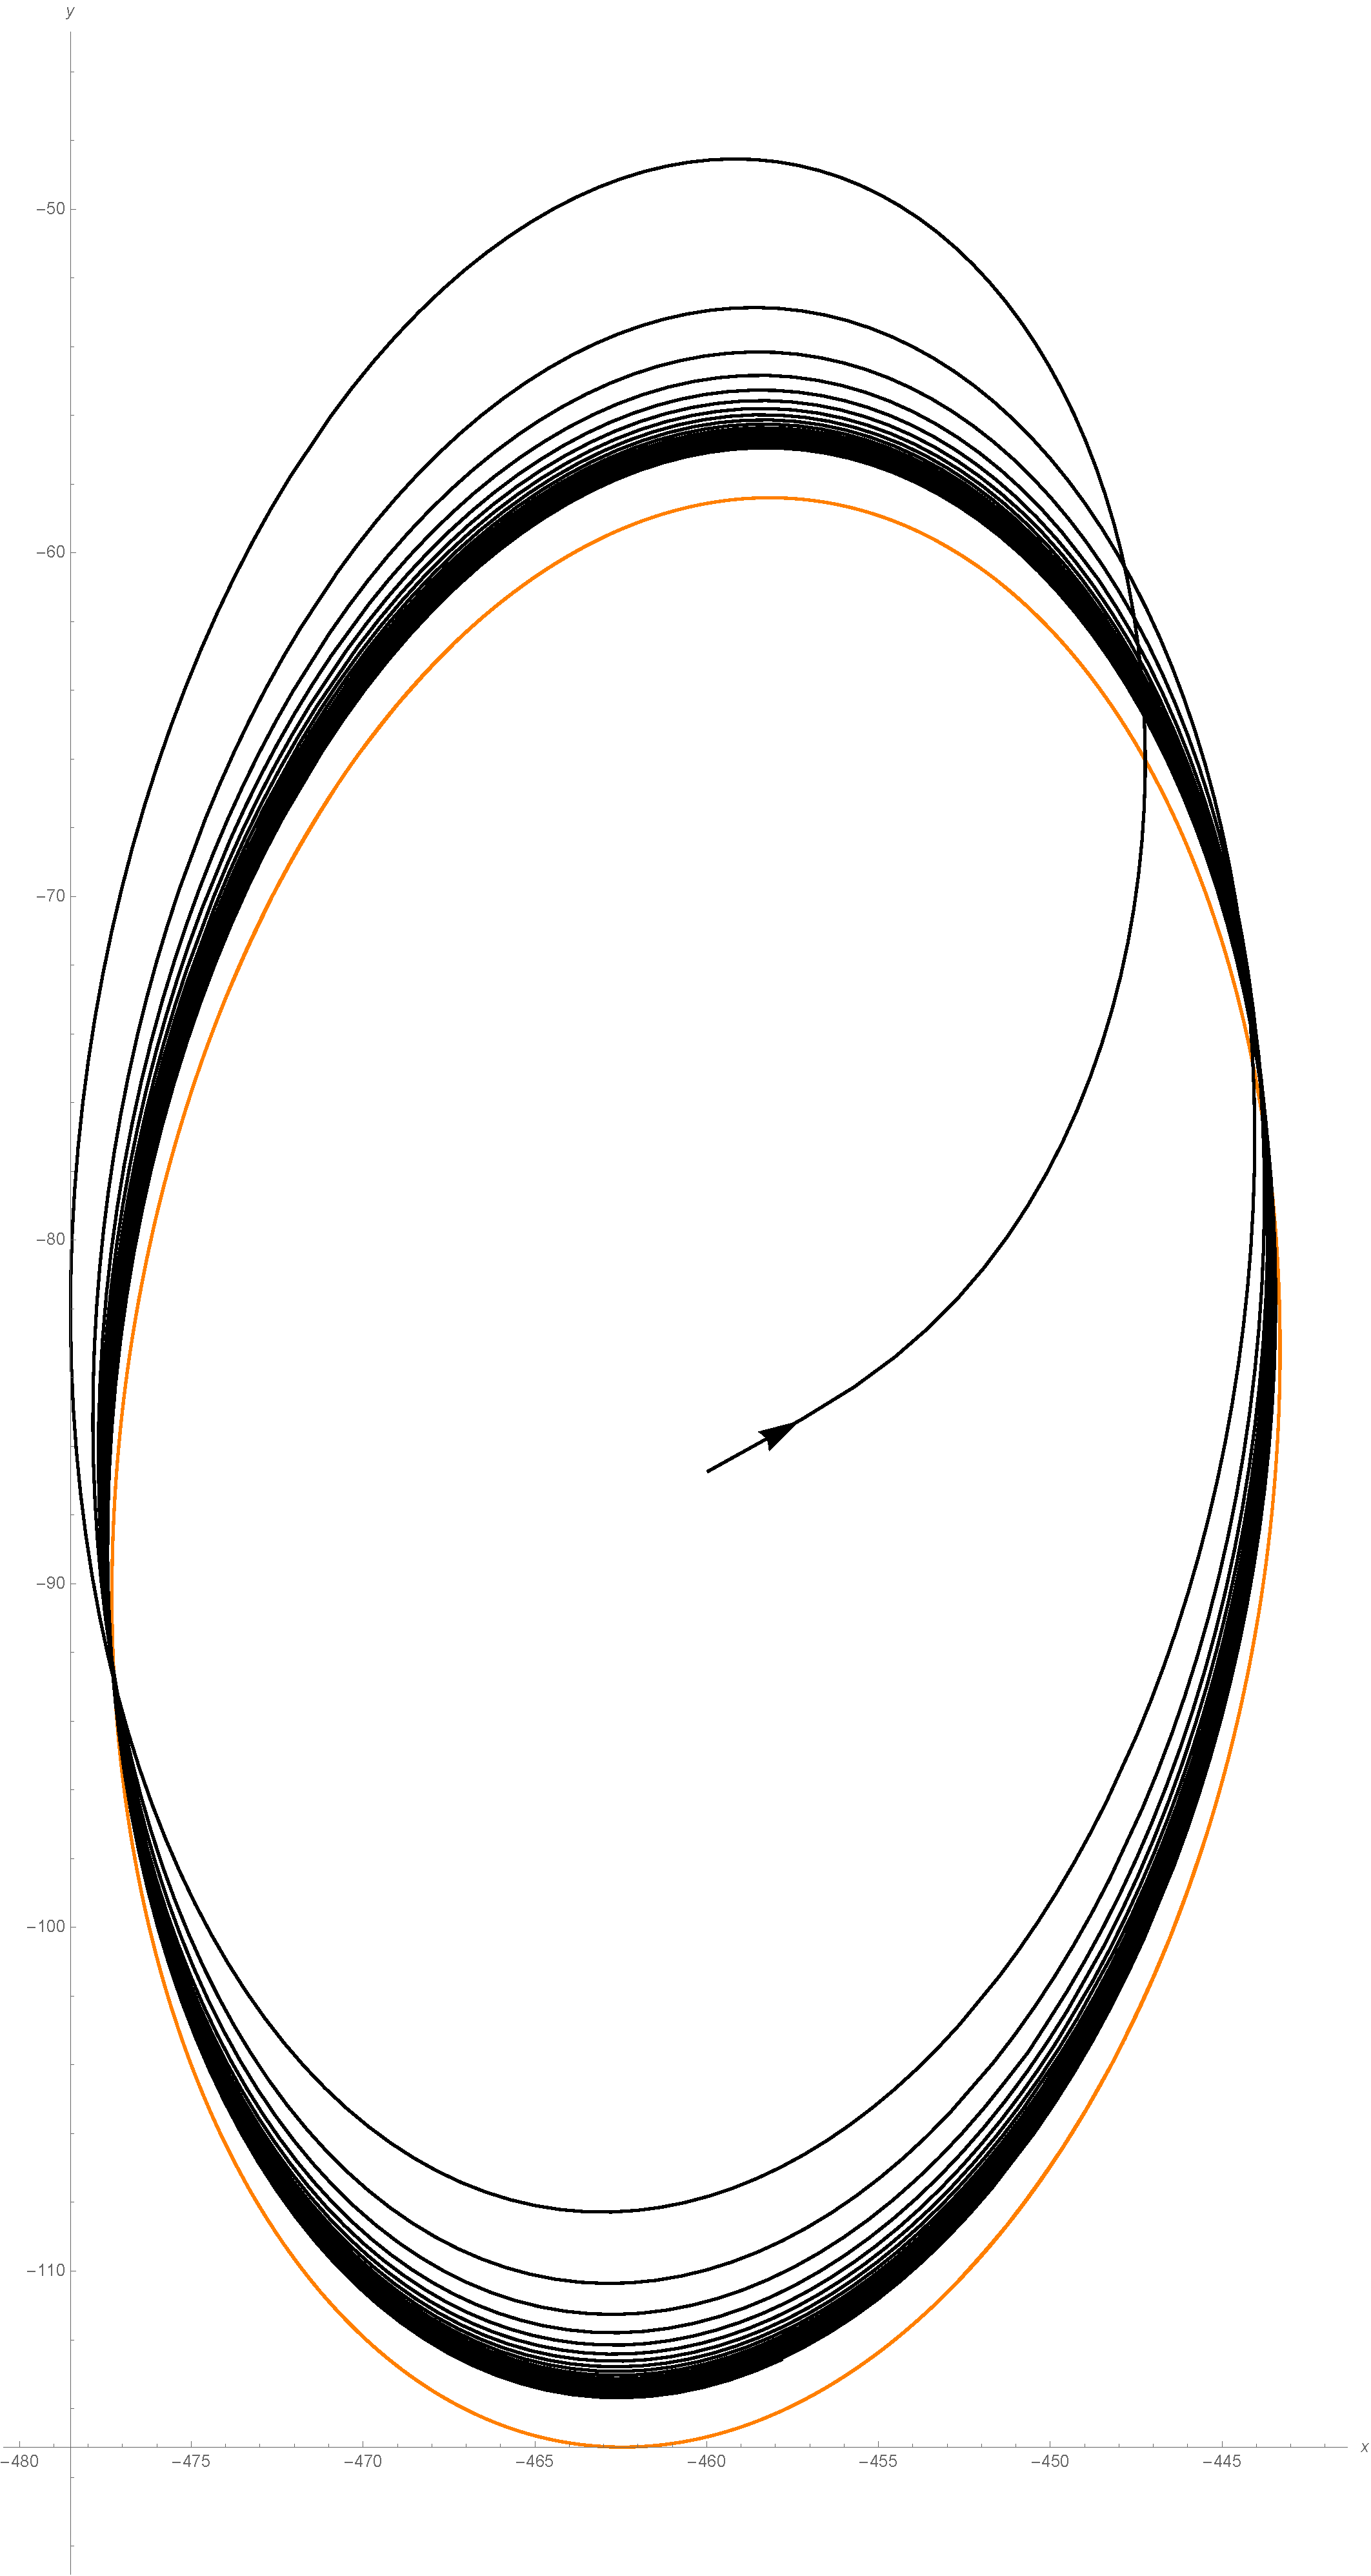
\includegraphics[width=0.4\textwidth]{ais1orbitpara}
    \caption{Parametric plot of (stable) solution corresponding to point F on bifurcation diagram, $\alpha = 1$ and $\omega=0.9$. $s=0.424264$ and $k=0.1$.}
    \label{fig: Stable parametric Point F}   
\end{figure}
\begin{figure}[h]%
\centering
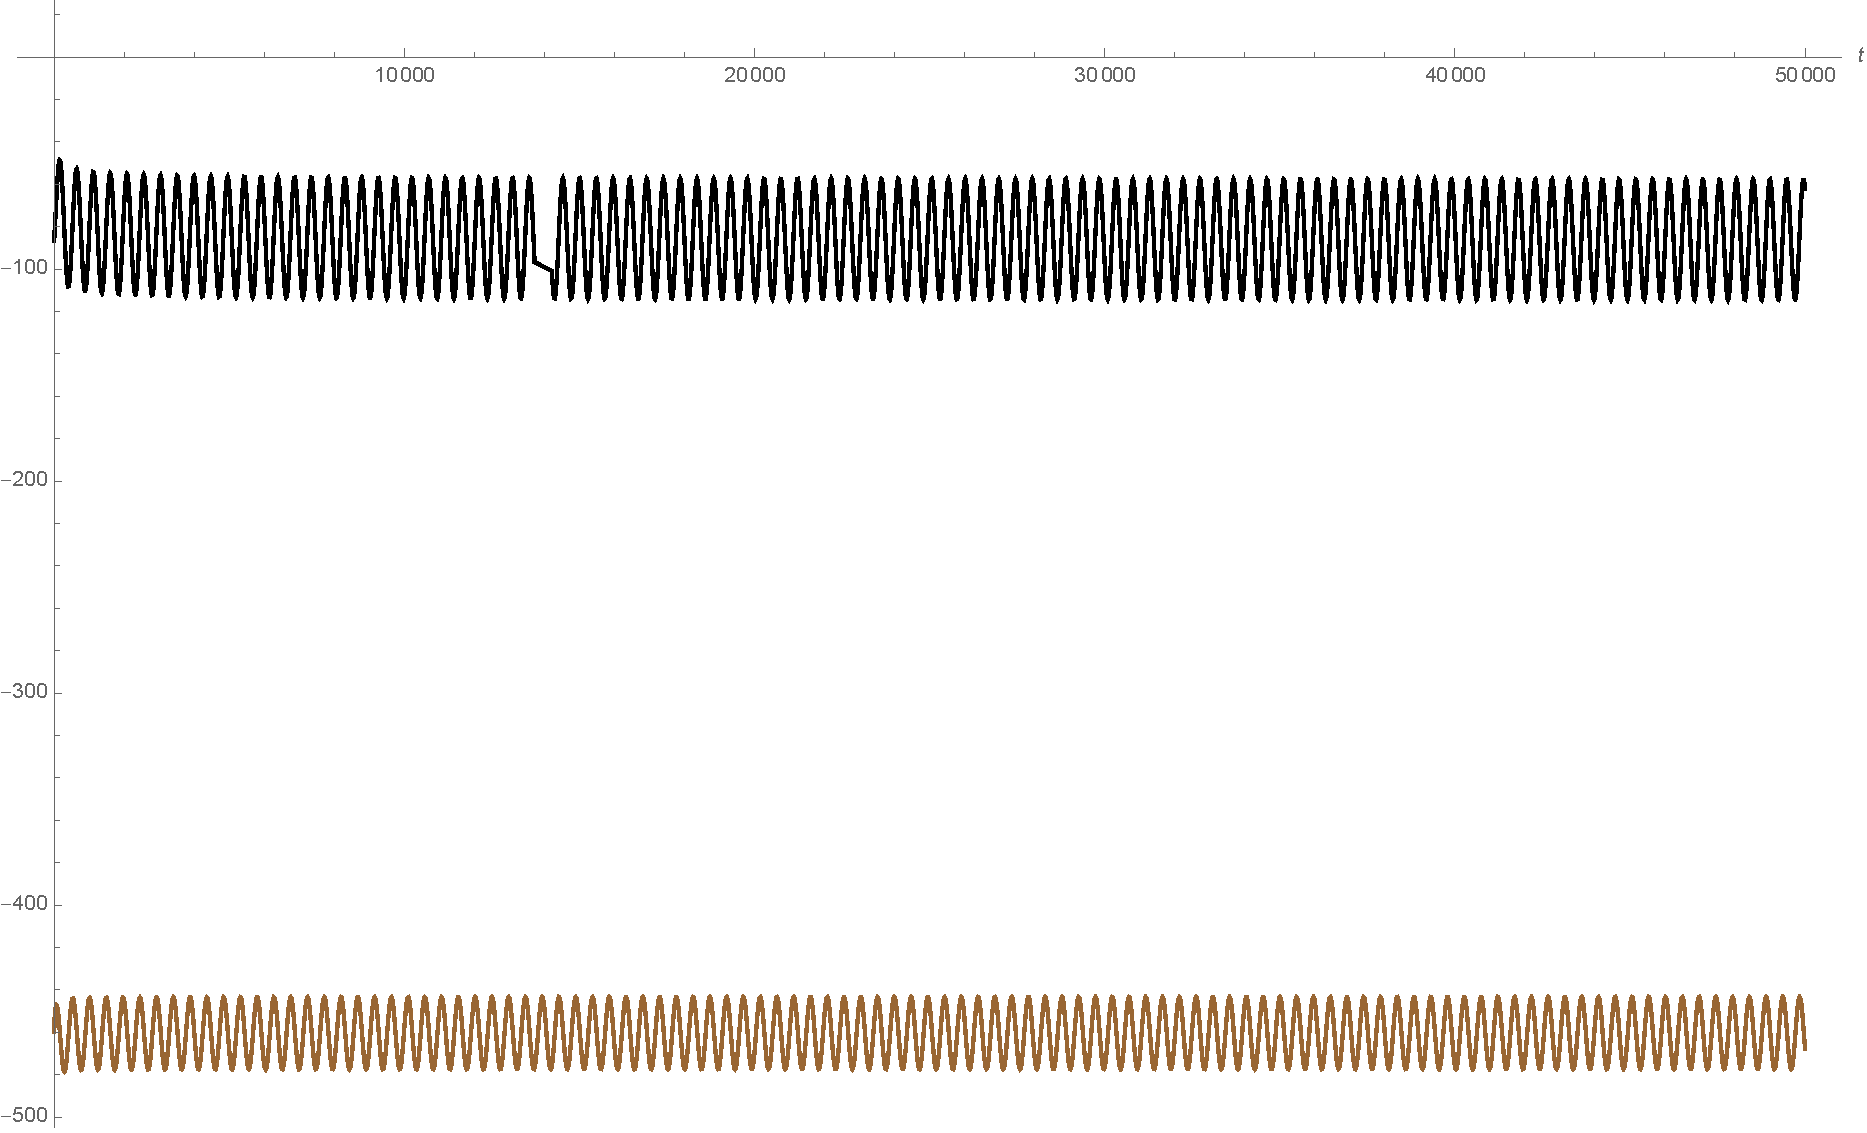
\includegraphics[width=0.42\textwidth]{ais1orbitplot}
    \caption{Plot of $x$ and $y$ vs time Stable case corresponding to point F on bifurcation diagram, $\alpha = 1$ and $\omega=0.9$. $s=0.424264$ and $k=0.1$.}
    \label{fig:Stable  Point F}
\end{figure}

\subsubsection{$9^{th}$ set of parameters: corresponding to point G in the bifurcation diagram.}\label{$9{th}$ set}
The parameter values, $\alpha = 1$, $Re_{s}=0.05$, $\omega=\frac{1}{\sqrt{2}}=s$ and $k=0$ correspond to point G (cf. Fig. \ref{fig:Bifurcation a vs w}), corresponding eigenvalues are: $\{-0.866025-0.5 i,-0.866025+0.5 i,-0.866025-0.5 i,-0.866025+0.5 i,0,0,0,0\}$.

The equilibrium points will be $\mathbf{x}_{eq}=
 \left(
\begin{array}{c}
-424.264 \\
y \\\end{array}
\right)$.

When the initial condition is \begin{align*}
X_{0}=&
\left(
x(0) ,
y(0) ,
{ }_{0}^{C}D_{t}^{\frac{1}{2}}x(0) ,
{ }_{0}^{C}D_{t}^{\frac{1}{2}}y(0) ,
{ }_{0}^{C}D_{t}^{1} x(0) ,
{ }_{0}^{C}D_{t}^{1}y(0) ,
{ }_{0}^{C}D_{t}^{\frac{3}{2}}x(0) ,
{ }_{0}^{C}D_{t}^{\frac{3}{2}}y(0)
\right)^T \\ =& \left(
 -423.693 ,
 c+0.835017 ,
 0.831797 ,
 0.260973 ,
 0.282803 ,
 0.726109 ,
 0.180962 ,
 0.150749 
\right)^T,
\end{align*}
(where c is some constant) we get the solution as shown in Fig.  \ref{fig: Unstable parametric Point G} and Fig. \ref{fig: Unstable  Point G}.

  \begin{figure}
  \centering
    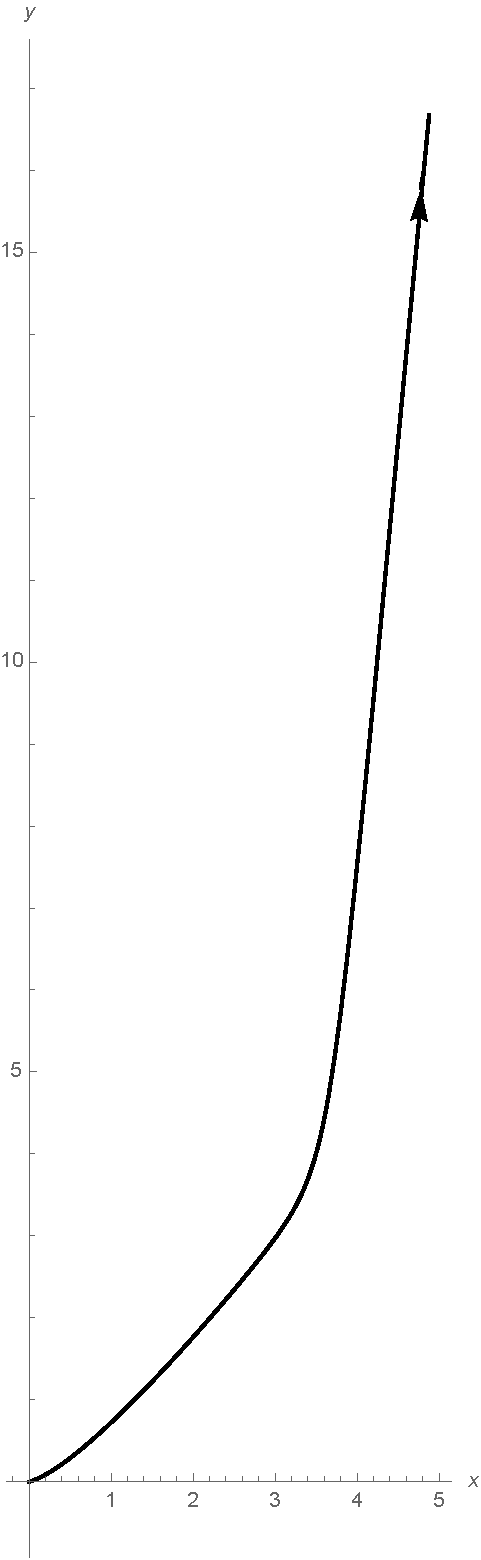
\includegraphics[width=0.18\textwidth]{ais1wisroot2Para}
    \caption{Parametric plot of (unstable) solution corresponding to point G on bifurcation diagram, $\alpha = 1$, $\omega=\frac{1}{\sqrt{2}}=s$ and $k=0$.}
    \label{fig: Unstable parametric Point G}   
\end{figure}
\begin{figure}[h]%
\centering
 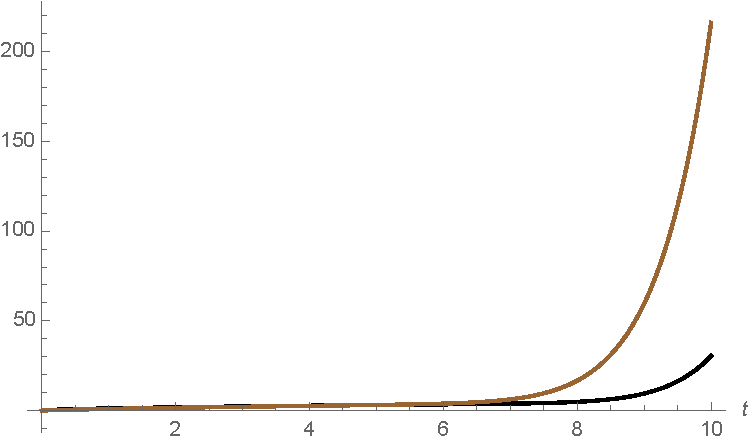
\includegraphics[width=0.4\textwidth]{ais1wisroot2Plot}
    \caption{Plot of $x$ and $y$ vs $t$ solution corresponding to point G on bifurcation diagram $\alpha = 1$, $\omega=\frac{1}{\sqrt{2}}=s$ and $k=0$}
    \label{fig: Unstable  Point G}
\end{figure}

% $9^{th}$ and $10^{th}$ sets of parameters have been solved using matrix variate Mittag Leffler functions as $A $ is a singular non-diagonalisable matrix. Here, we have taken the solution of the system as, 
%$$X(t)= \left(\sum _{j=1}^{\infty} \frac{t^{j/2}A^{j}}{\Gamma \left(\frac{j}{2}+1\right)}\right)X_{0}$$
%We consider the first $10$ terms of the series for the plot.

It may be noted that $0$ is a repeated eigenvalue with multiplicity four, and the system is unstable.

\subsubsection{$10^{th}$ set of parameters: corresponding to point H in the bifurcation diagram.}\label{$10^{th}$ set}
Let : $\alpha = 4$, $Re_{s}=0.05$, $\omega=\frac{1}{\sqrt{2}}=s$ and $k=0$. This corresponds to point H, which is on the boundary line in Fig.\ref{fig:Bifurcation a vs w}.

The eigenvalues corresponding to these conditions are:$ \{-1.93185,-1.93185,-0.517638,-0.517638,0,0,0,0\}$.
Hence, $0$ is a repeated eigenvalue with multiplicity 4 which makes the system unstable. 
$$\mathbf{x}_{eq}=
\left(
\begin{array}{c}
-848.528 \\
y \\
\end{array}
\right)$$
If the initial conditions are:\begin{align*}
X_{0}=&
\left(
x(0) ,
y(0) ,
{ }_{0}^{C}D_{t}^{\frac{1}{2}}x(0) ,
{ }_{0}^{C}D_{t}^{\frac{1}{2}}y(0) ,
{ }_{0}^{C}D_{t}^{1} x(0) ,
{ }_{0}^{C}D_{t}^{1}y(0) ,
{ }_{0}^{C}D_{t}^{\frac{3}{2}}x(0) ,
{ }_{0}^{C}D_{t}^{\frac{3}{2}}y(0)
\right)^T \\ =& \left(
 -848.358 ,
 c+0.54952 ,
 0.77192,
 0.134856,
 0.784236,
 0.727202,
 0.171545,
 0.530859 
\right)^T,
\end{align*}
where c is a constant, we get the solution as depicted in Fig.\ref{fig:Unstable parametric Point H} and Fig.\ref{fig: Unstable  Point H}.
   \begin{figure}
  \centering
    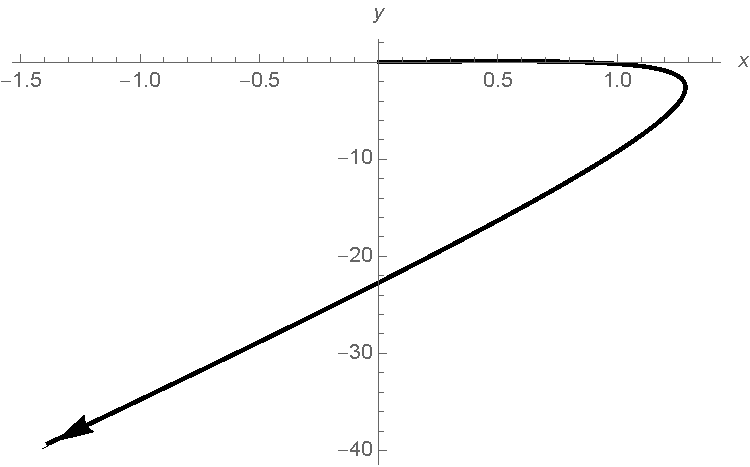
\includegraphics[width=0.4\textwidth]{ais4wisroot2}
    \caption{Parametric plot of (unstable) solution corresponding to point H on bifurcation diagram $\alpha = 4$, $\omega=\frac{1}{\sqrt{2}}=s$ and $k=0$.}
    \label{fig:Unstable parametric Point H}   
 
\end{figure}

\begin{figure*}[h]%
\centering
 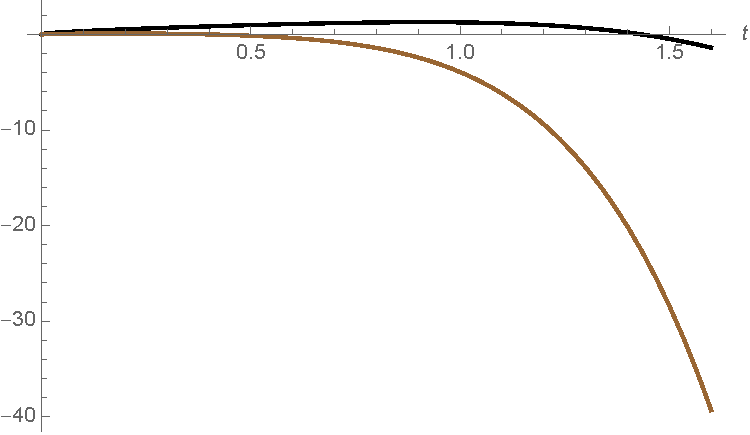
\includegraphics[width=0.4\textwidth]{ais4wisroot2Plot}
    \caption{Plot of $x$ and $y$ vs $t$ corresponding to point H on bifurcation diagram $\alpha = 4$, $\omega=\frac{1}{\sqrt{2}}=s$ and $k=0$.}
    \label{fig: Unstable  Point H}
\end{figure*}






%------------------------------------------------------------------------------------------------- 
\section{Conclusion}\label{conclusion}
The Maxey-Riley (M-R) equation is an important application of fractional calculus \cite{kobayashi2005stability}. In this paper, we provide accurate expressions for the equilibrium points of M-R equations, and perform their stability analysis. We note that the characteristic equation of this system is independent of the shear flow and stagnation flow. Further, we give explicit solutions in terms of Mittag-Leffler functions.

We highlight the existence of singular points in the solution trajectories of the M-R equation, a novel feature of fractional ordered dynamics. More research is needed for gaining insight of the physical meaning of such self-intersecting trajectories.

\section*{Data Availability Statement}
Data sharing not applicable to this article as no datasets were generated or analysed during the current study.

\backmatter
%%===========================================================================================%%

%%===========================================================================================%%

\bibliography{sn-bibliography}% common bib file
%% if required, the content of .bbl file can be included here once bbl is generated
%%\input sn-article.bbl
%% Default %%
%%\input sn-sample-bib.tex%
\end{document}

